\chapter{Supplementary figures}
\label{app:figures}

% 3 - LOCUS CHAPTER

\begin{figure}
	\centering
	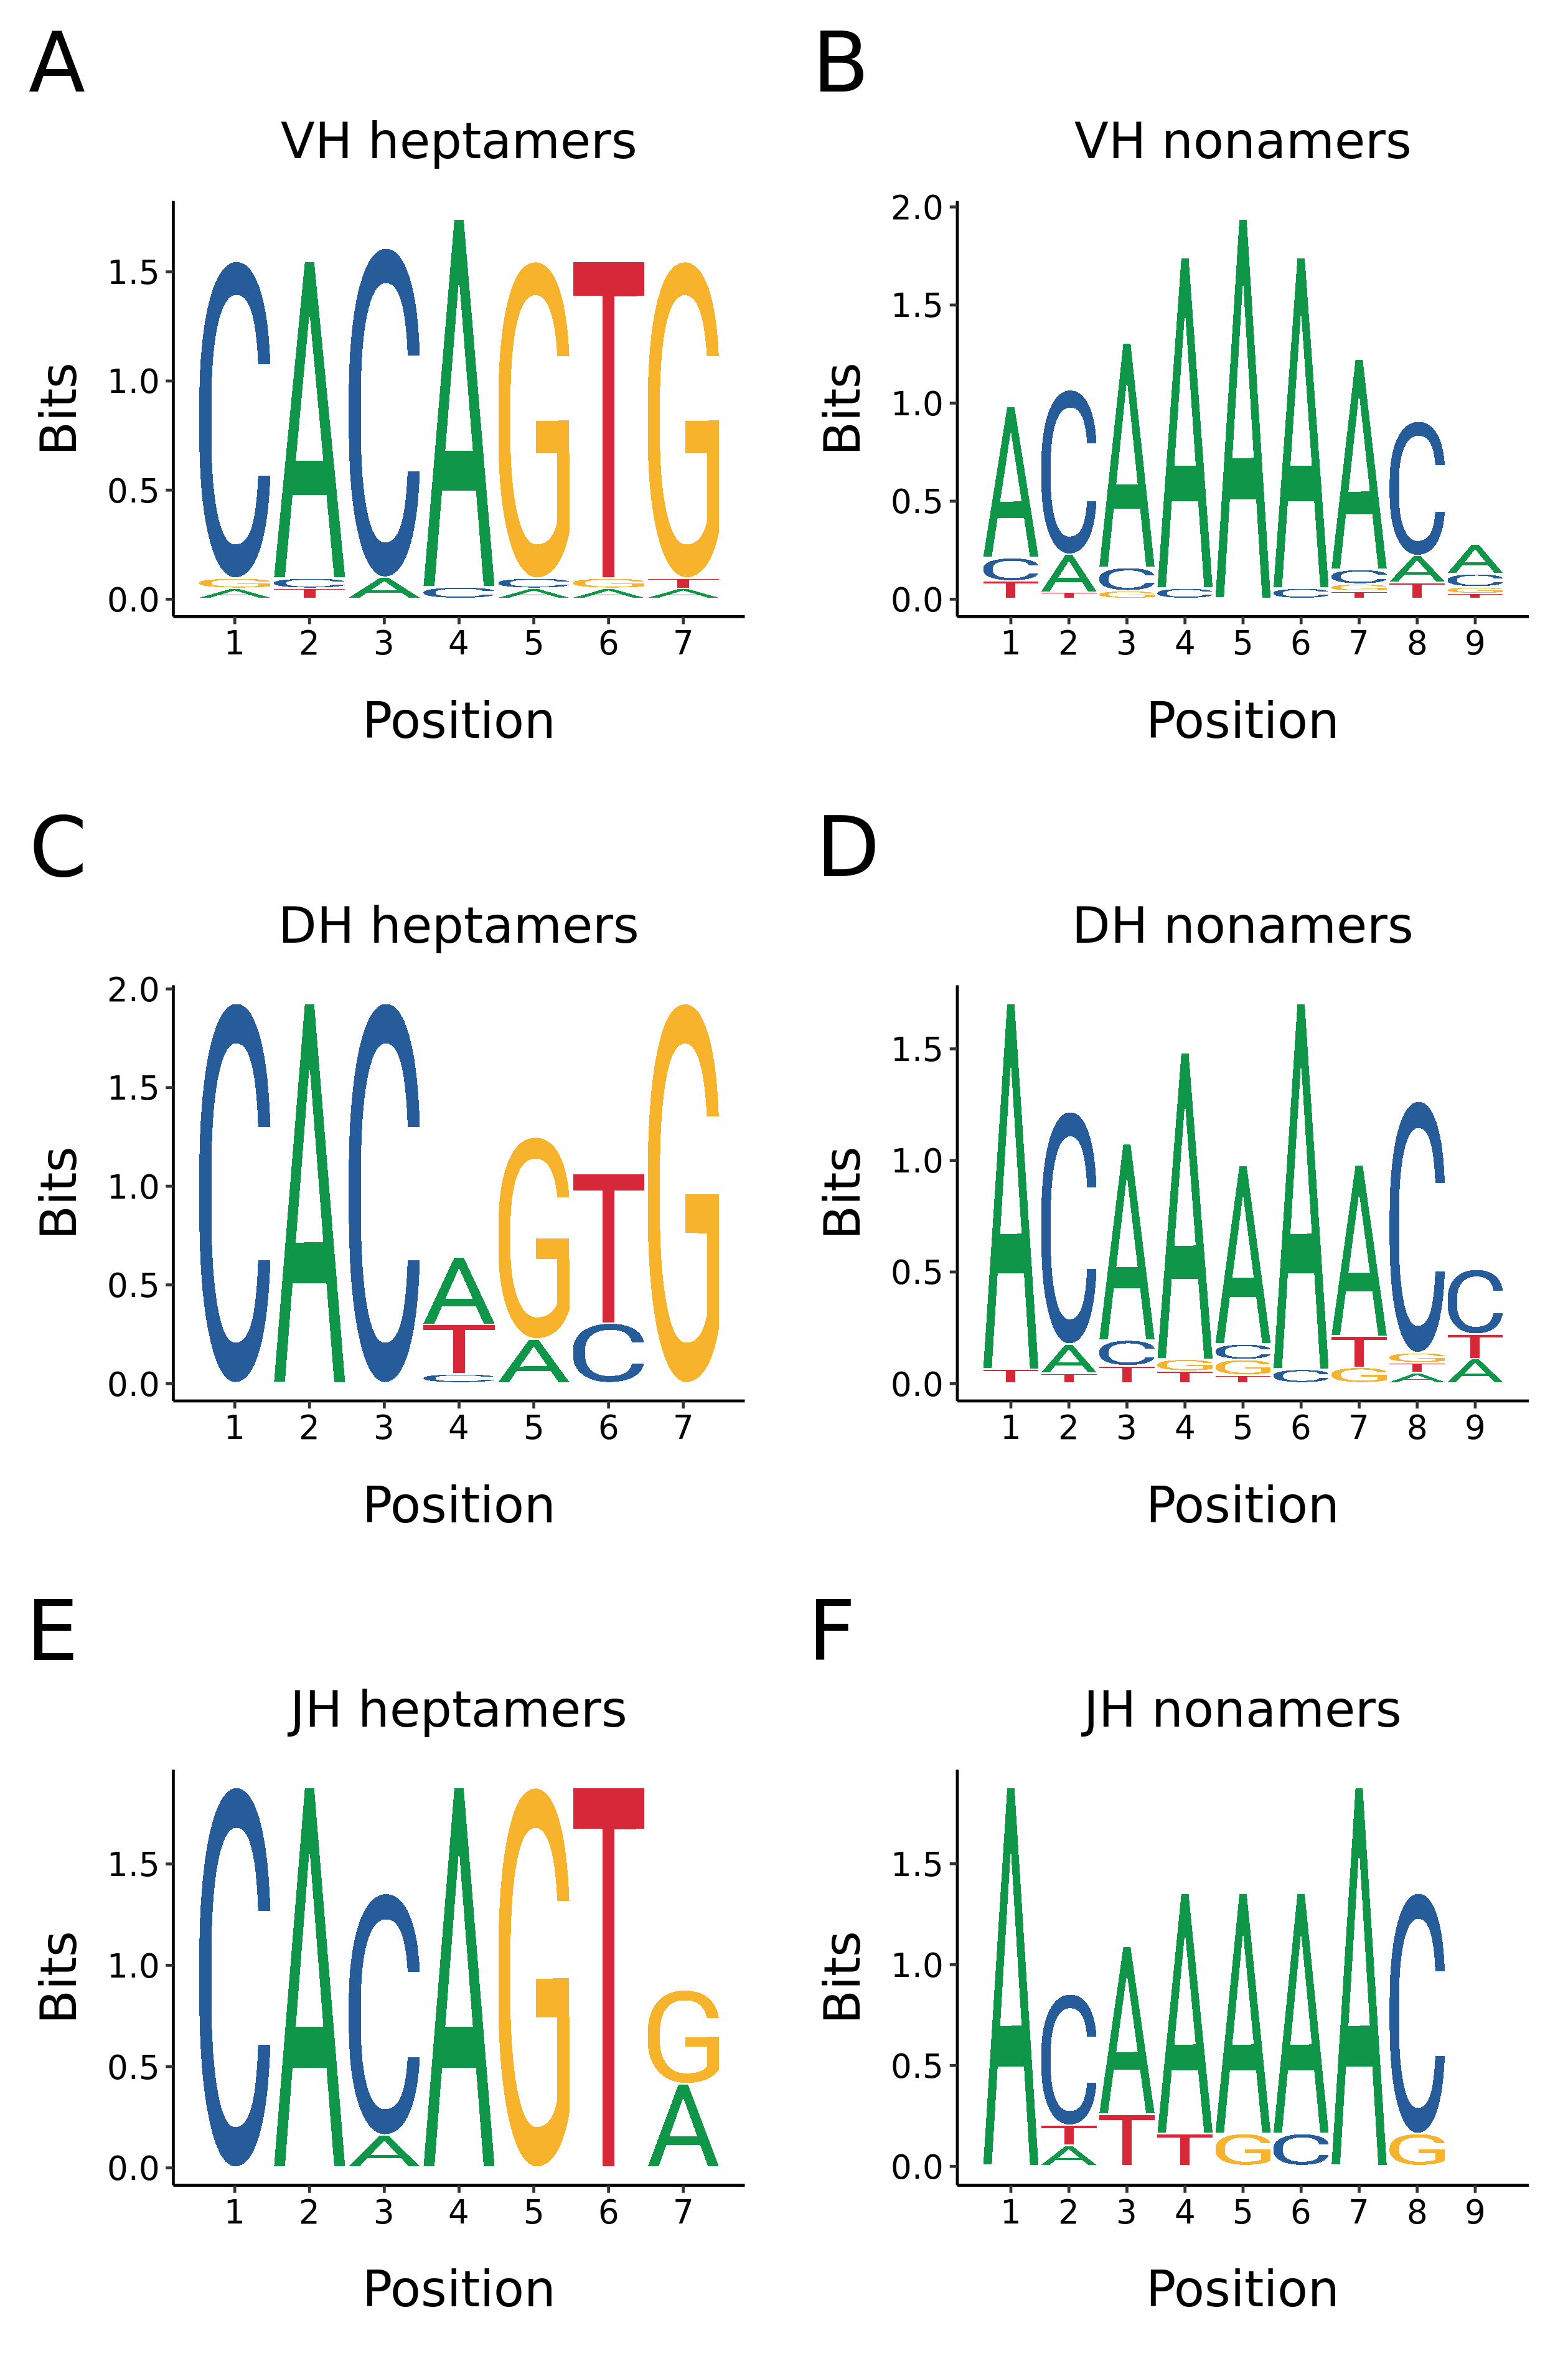
\includegraphics[width=0.9\textwidth]{_Figures/png/nfu-rss-seqlogo-sep}
	\caption[\Nfu recombination signal sequences by segment type]{\textbf{\Nfu recombination signal sequences by segment type:} Sequence composition of conserved heptamer (A,C,E) and nonamer (B,D,F) sequences from \Nfu heavy-chain RSSs associated with \vh (A,B), \dh (C,D) or \jh (E,F) gene segments.}
	\label{fig:nfu-rss-seqlogo-sep}
\end{figure}

\begin{figure}
	\centering
	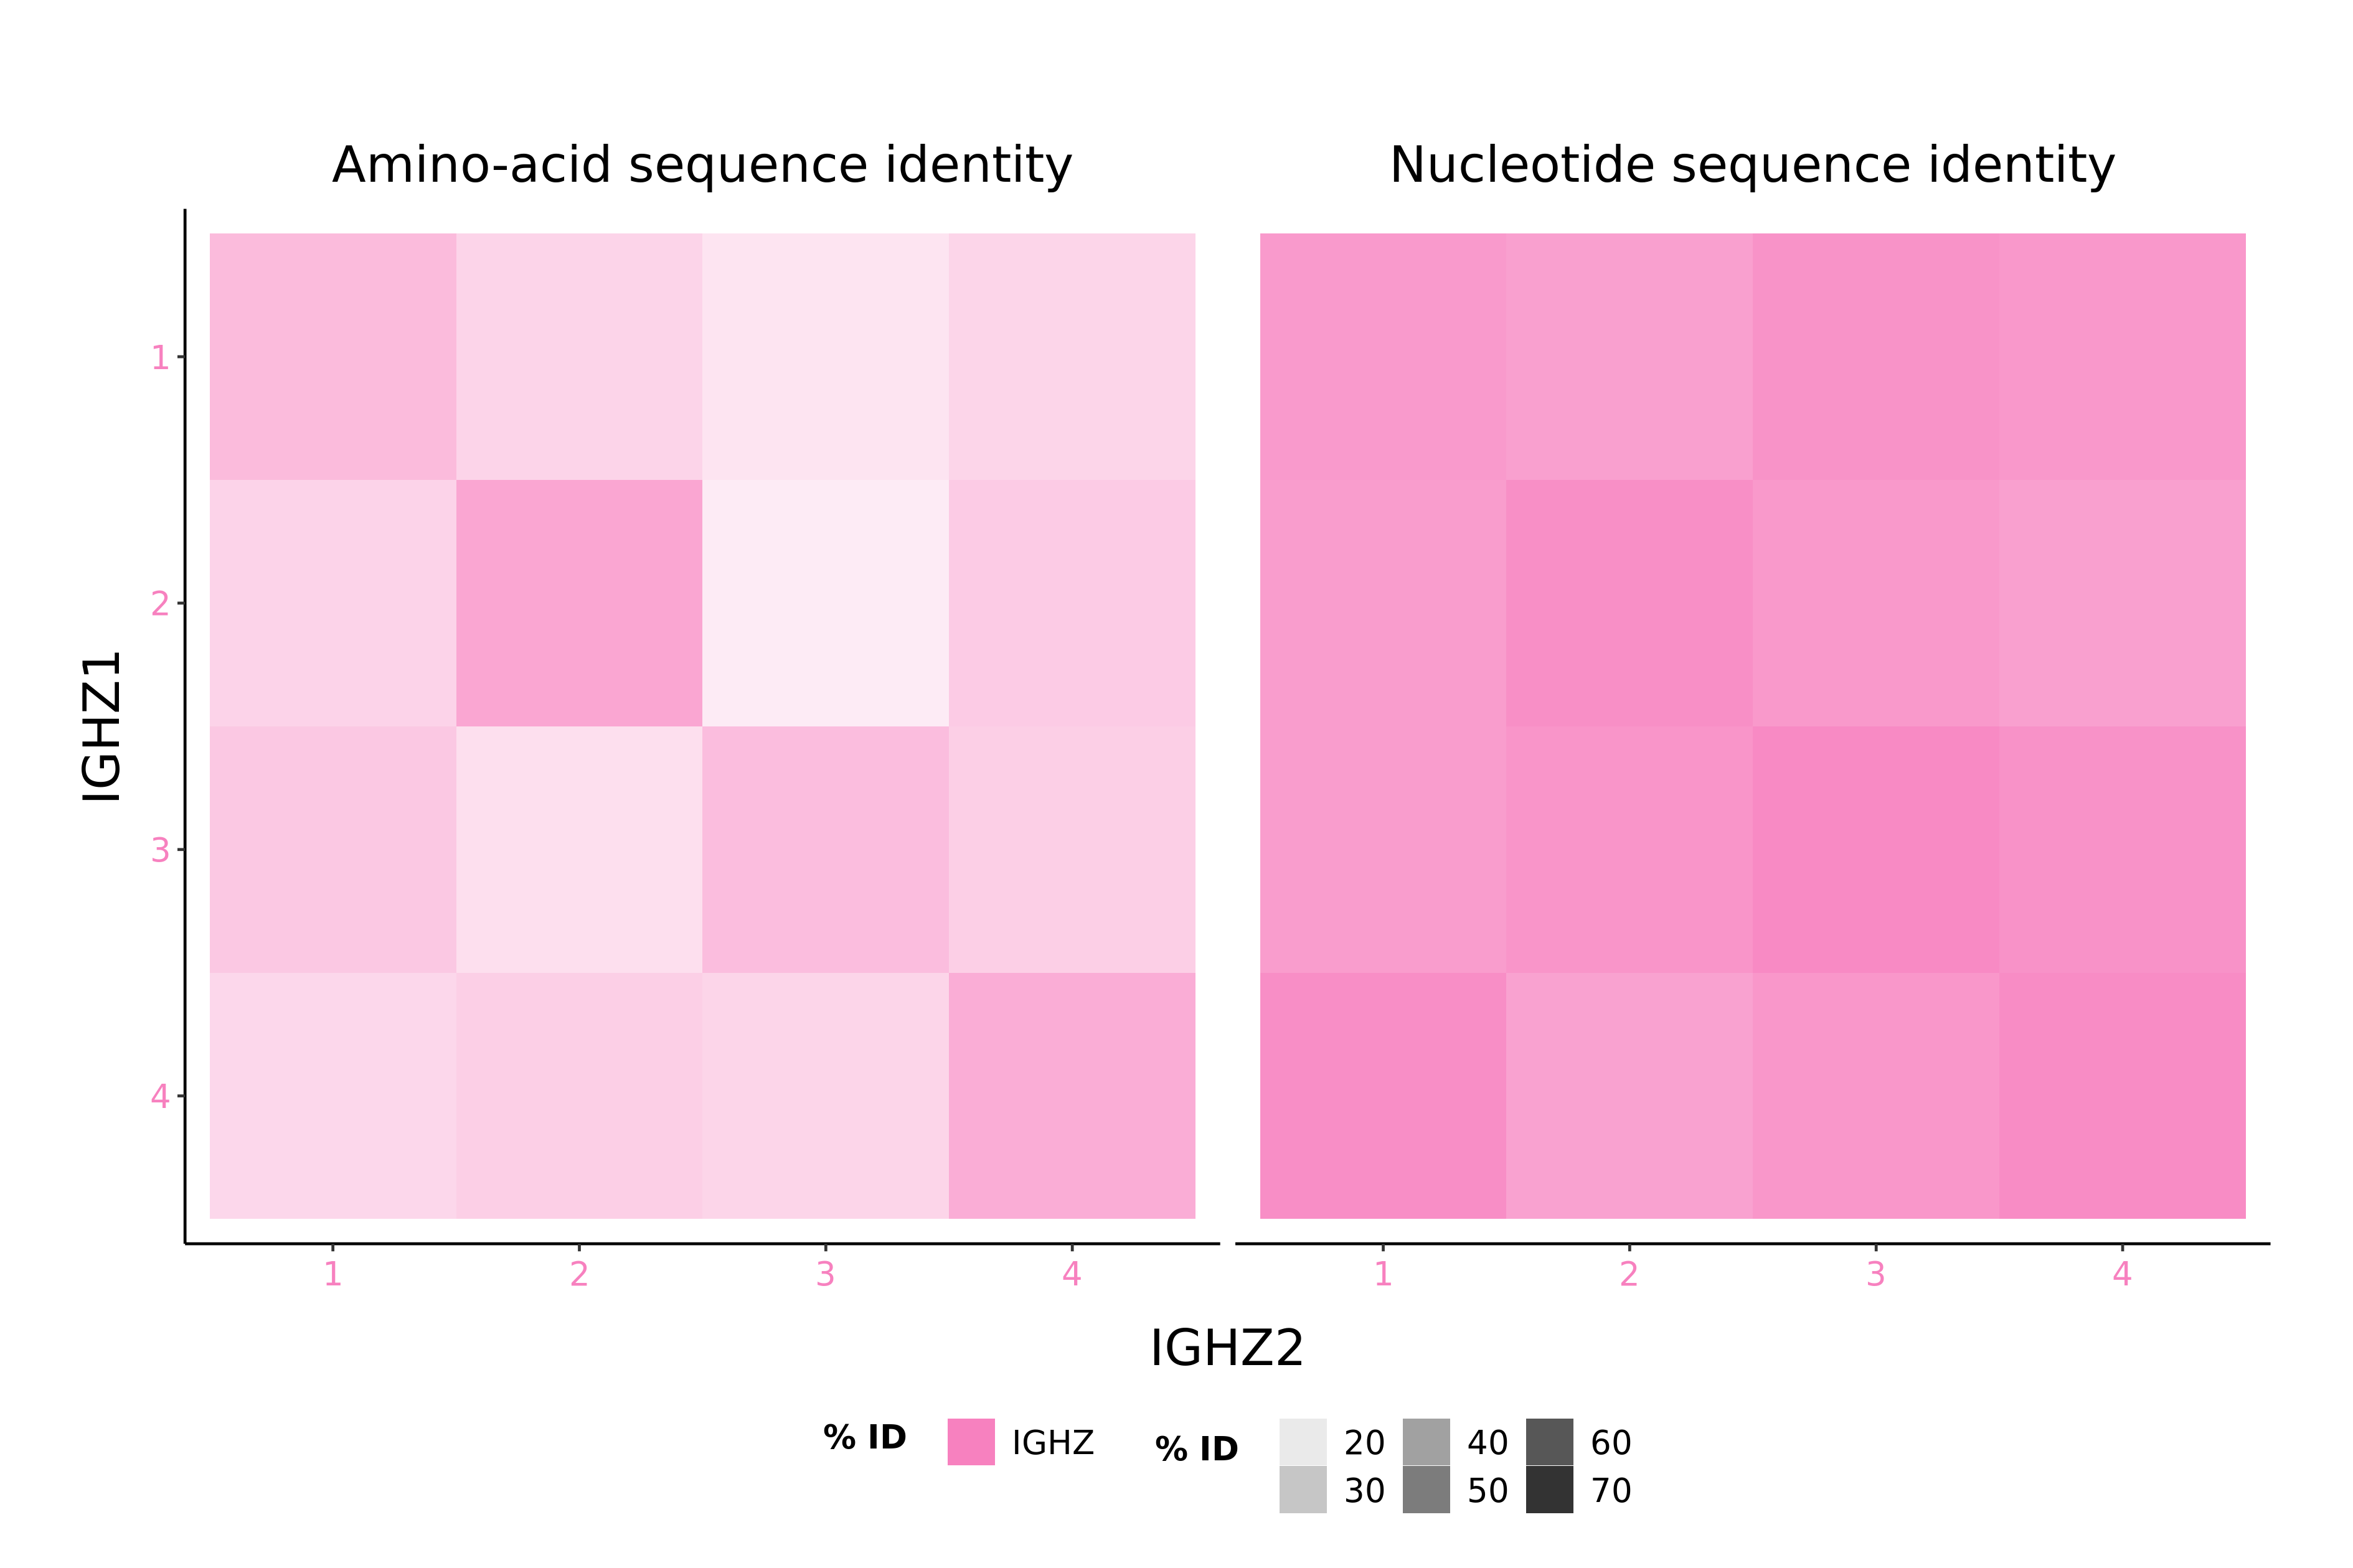
\includegraphics[width=0.8\textwidth]{_Figures/png/xma-new-cz-aln}
	\caption[Sequence similarity between \igh{Z} constant-regions in \Xma]{\textbf{Sequence similarity between \igh{Z} constant-regions in \Xma:} Heatmap of percentage sequence identity between amino-acid (right) and nucleotide (left) sequences of \cz{} exons from the two \Xma \igh{Z} constant regions, calculated using pairwise Needleman-Wunsch global alignments.} % TODO: Combine isotype and identity legends
	\label{fig:xma-cz-aln}
\end{figure}

	\begin{figure}
	\centering
	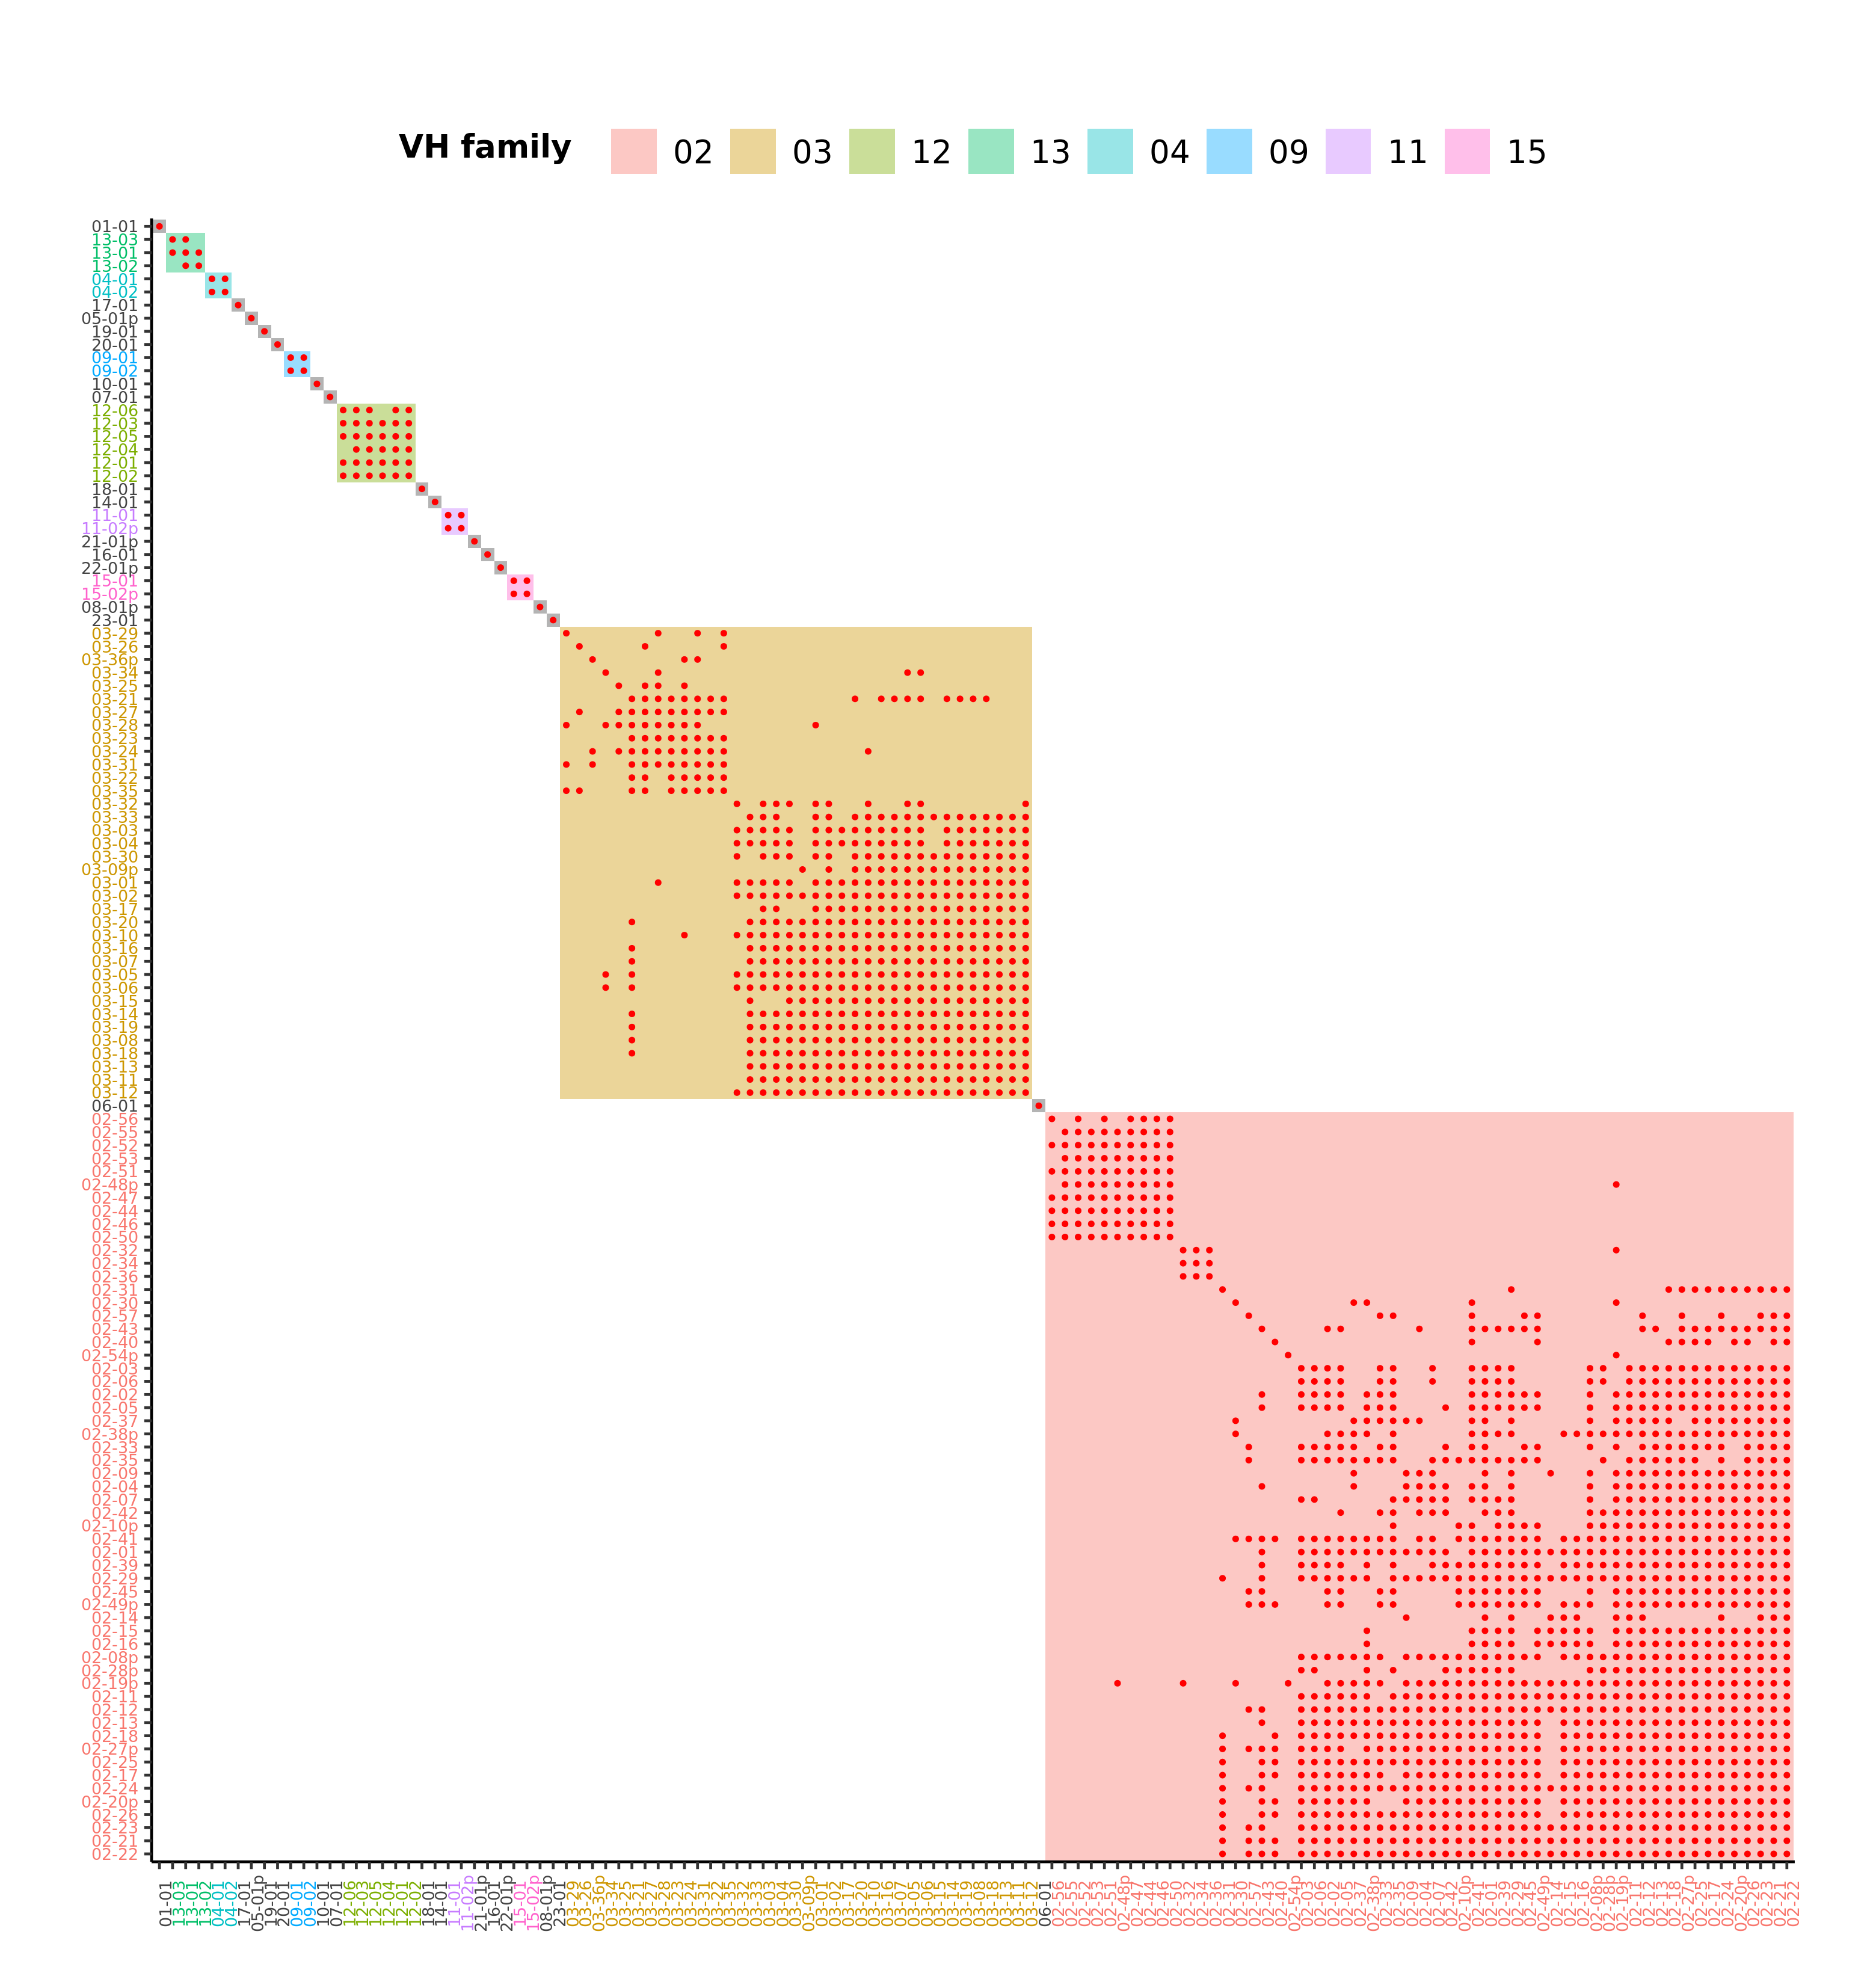
\includegraphics[width=\textwidth]{_Figures/png/xma-vh-families-map}
	\caption[Heatmap of \vh families in the in \Xma \textit{IgH} locus]{\textbf{Heatmap of \vh families in the in \Xma (\textit{IgH}) locus:} Heatmap of family relationships among \Xma \vh segments, with coloured shading indicating families and red dots indicating pairwise nucleotide sequence identity of at least 80\%. \vh families containing multiple segments are uniquely coloured, while single-segment families are in grey.}
	\label{fig:xma-vh-families-map}
	\end{figure}

	\begin{figure}
	\centering
	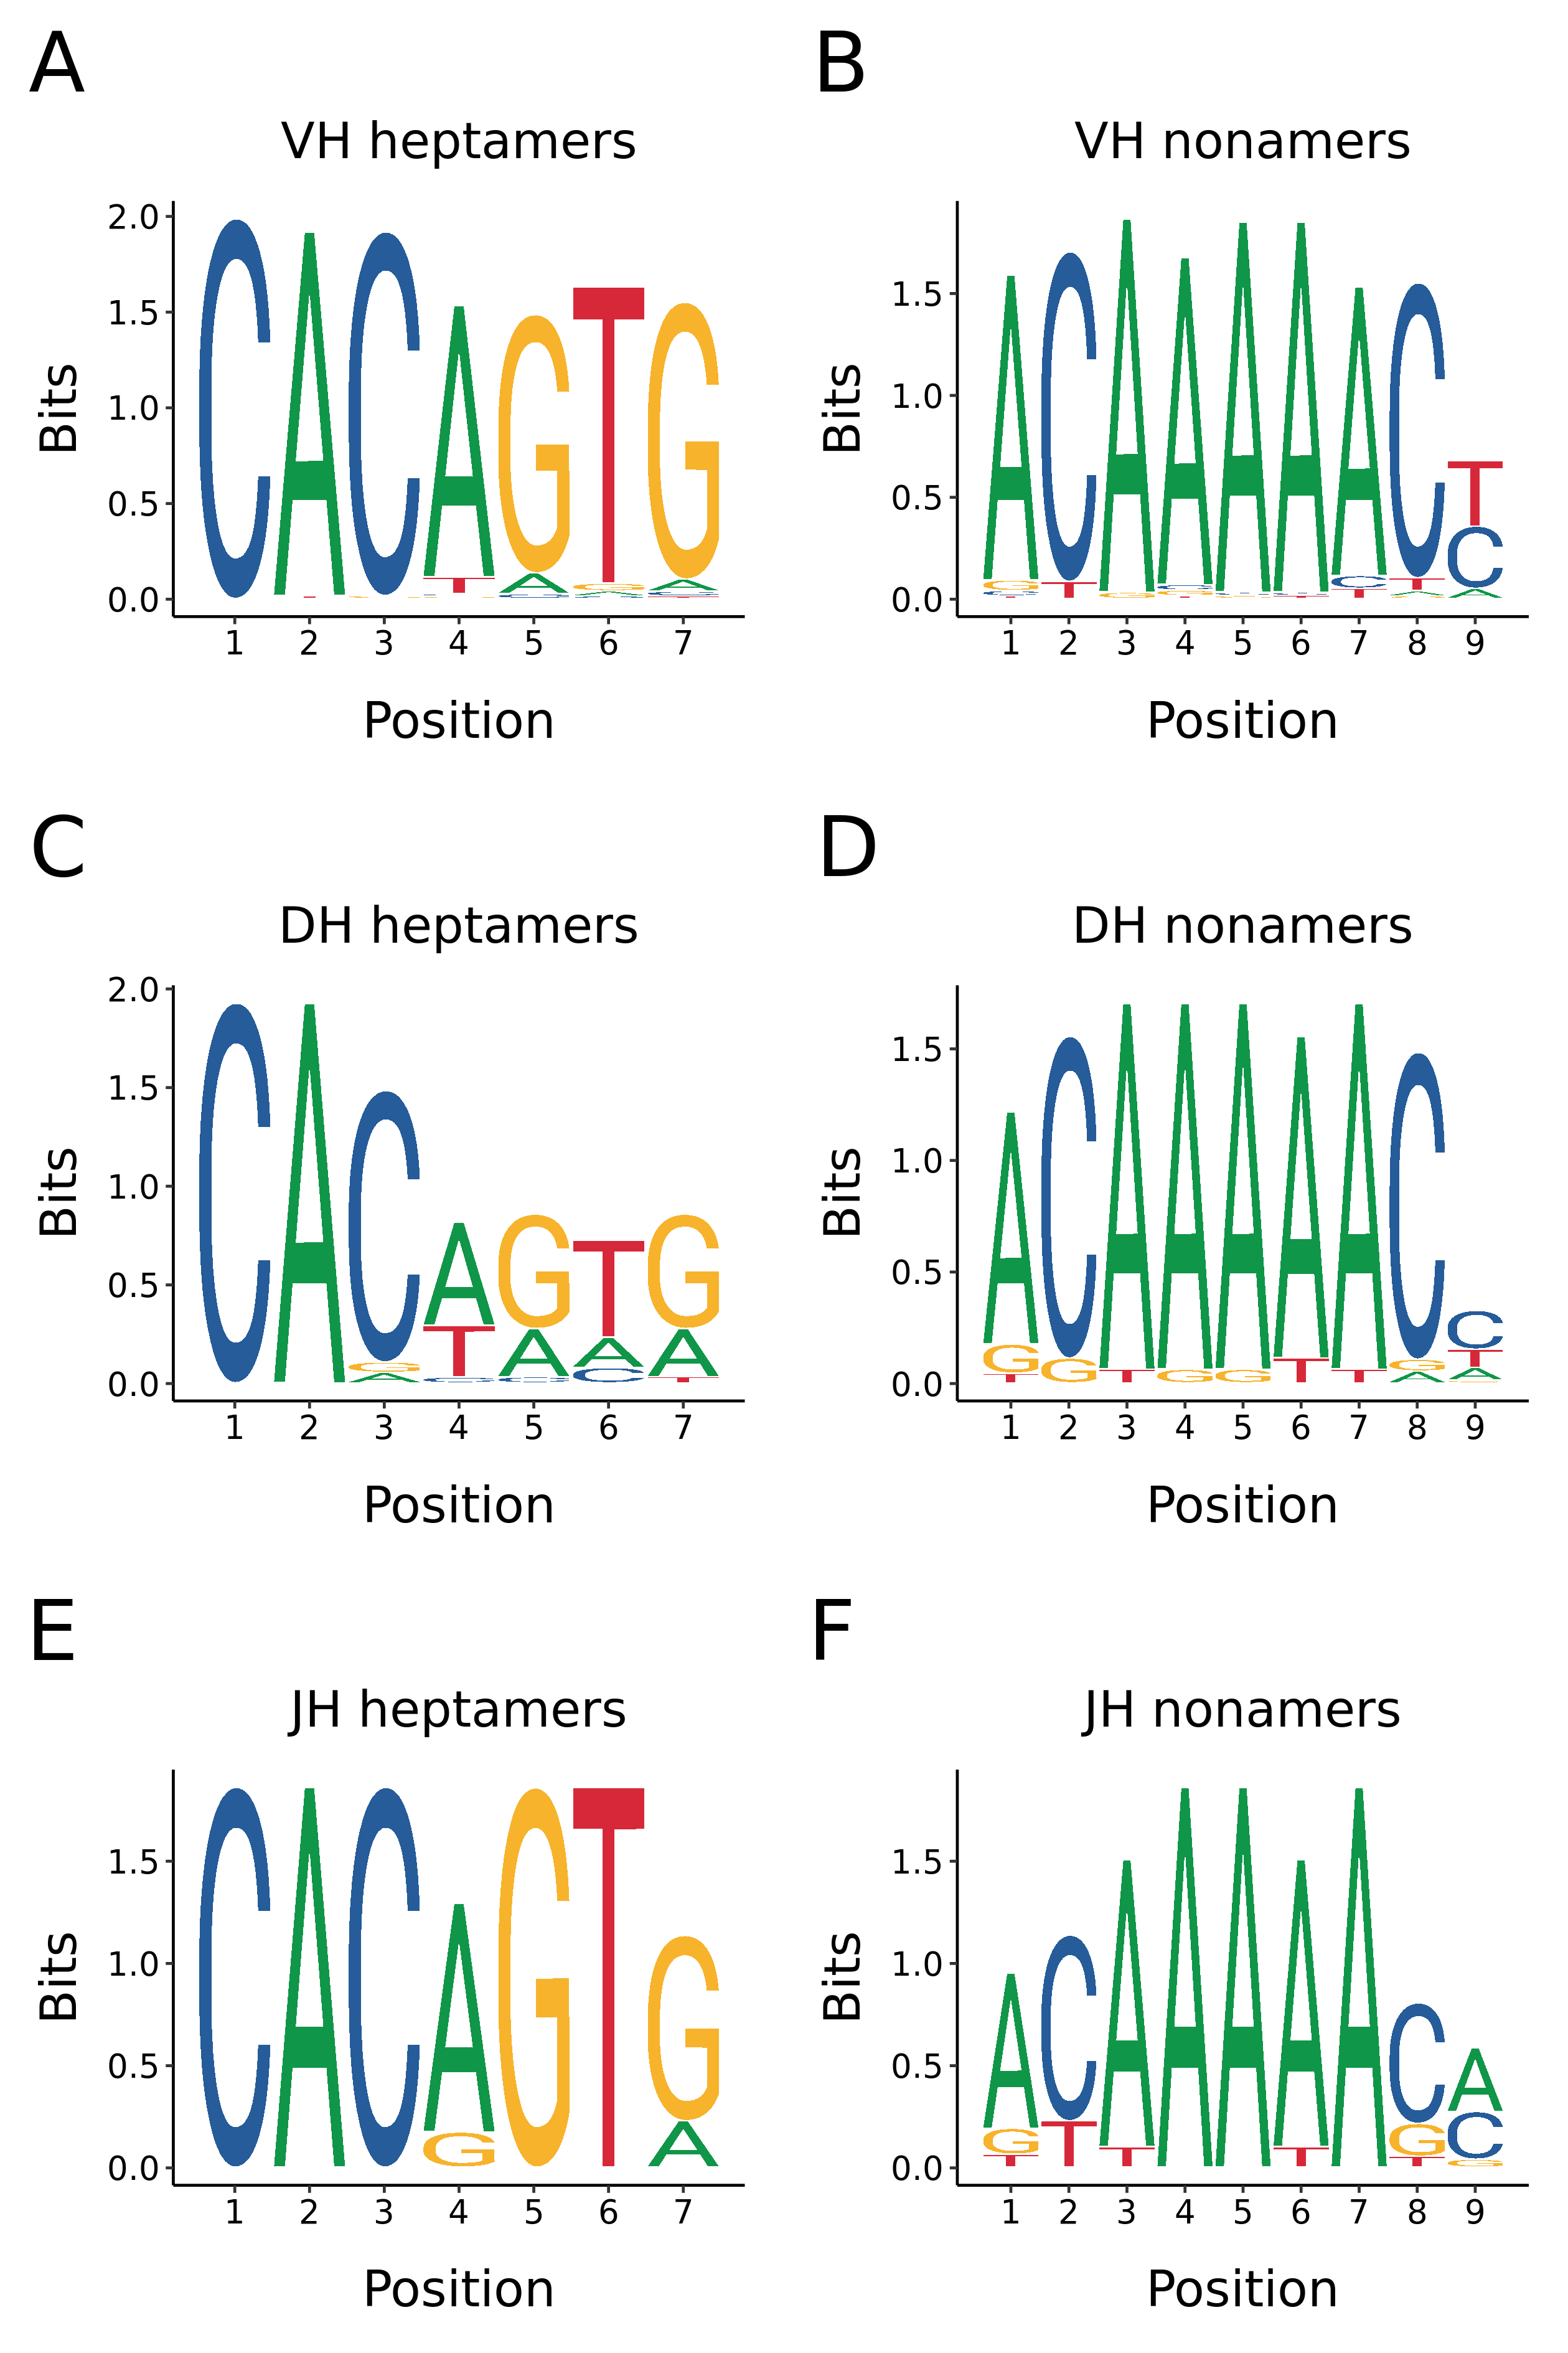
\includegraphics[width=0.9\textwidth]{_Figures/png/xma-new-rss-seqlogo-sep}
	\caption[\Xma recombination signal sequences by segment type]{\textbf{\Xma recombination signal sequences by segment type:} Sequence composition of conserved heptamer (A,C,E) and nonamer (B,D,F) sequences from \Xma heavy-chain RSSs associated with \vh (A,B), \dh (C,D) or \jh (E,F) gene segments.}
	\label{fig:xma-rss-seqlogo-sep}
	\end{figure}
	
% 4 - IGSEQ CHAPTER

\begin{figure}
\centering
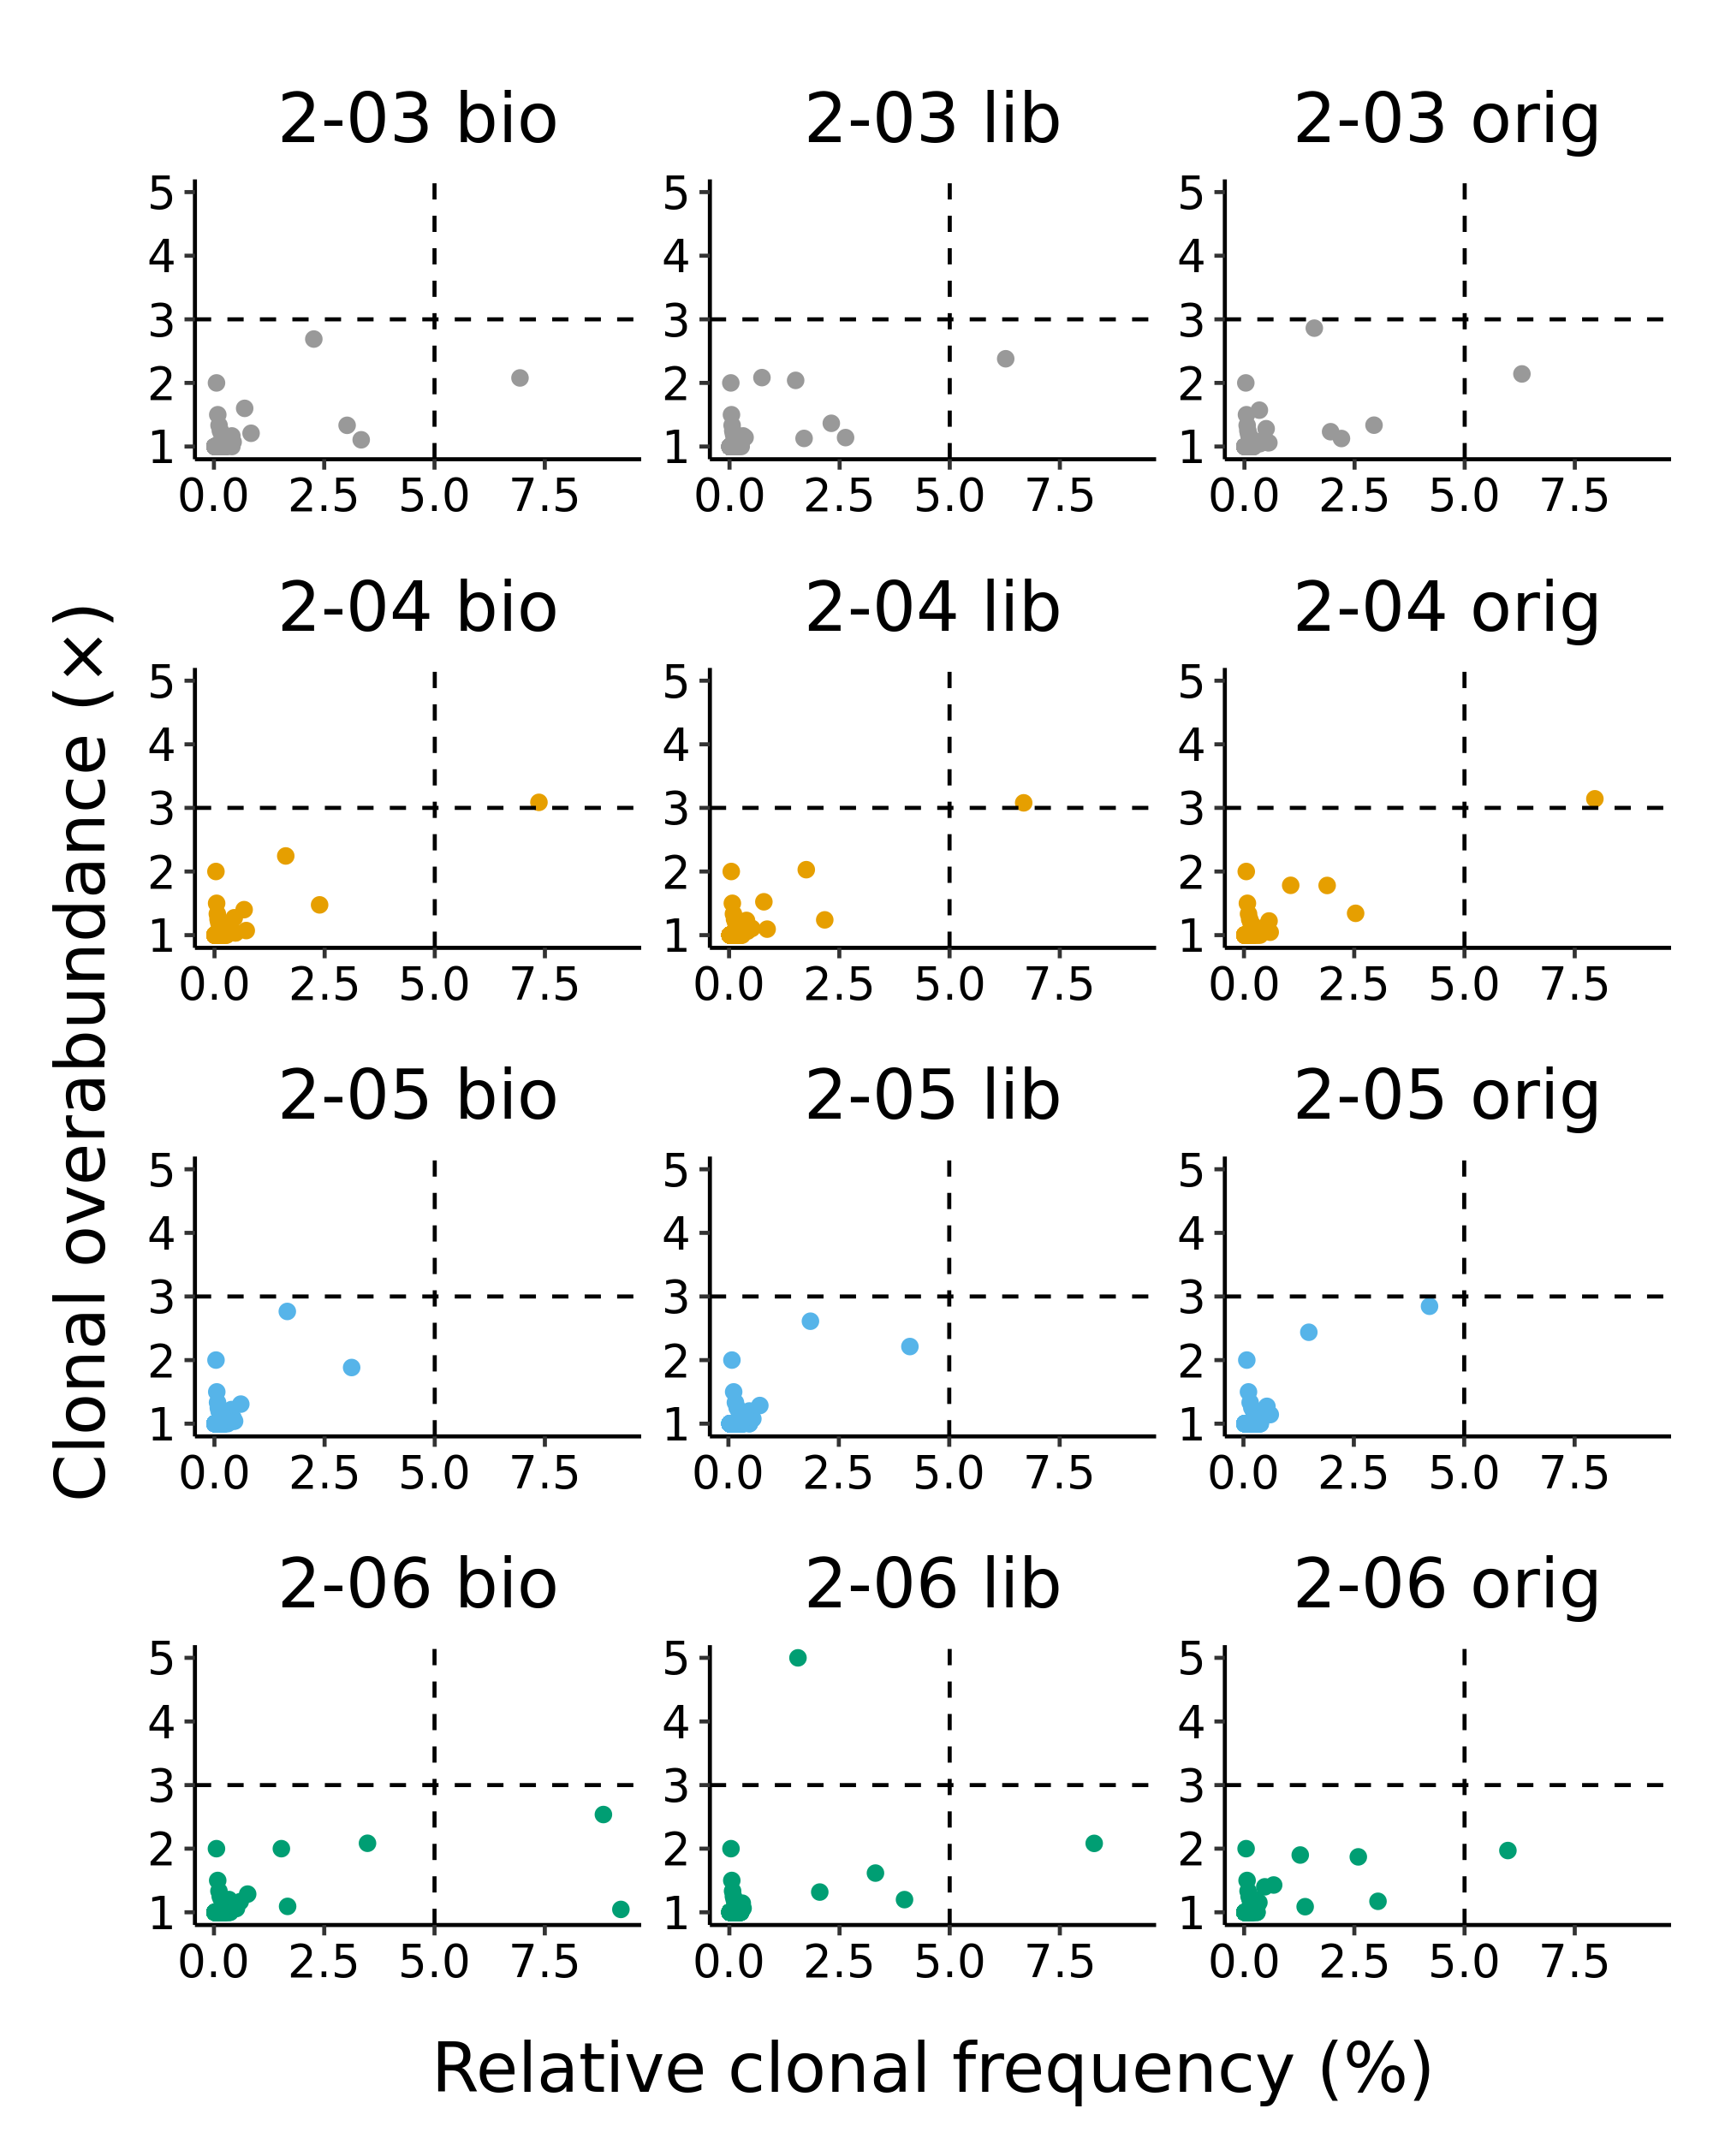
\includegraphics[width=0.8\textwidth]{_Figures/png/pilot-clones-expansions-rep}
\caption[Clonal expansions in \Nfu pilot repertoires]{\textbf{Clonal expansions in \Nfu pilot repertoires}: Scatter plots of clonal abundance for each replicate in the pilot \igseq dataset, measured in terms of the proportion of unique sequences in the repertoire ($x$-axis) and the abundance relative to the next-largest clone ($y$-axis). Thresholds for identifying clonal expansions (5\,\% and 3-fold for the $x$- and $y$-axis, respectively) suggested by Rosenfeld \textit{et al.} \parencite{rosenfeld2018clonesize}.}
\label{fig:igseq-pilot-clones-expansions-rep}
\end{figure}

\begin{figure}
\centering
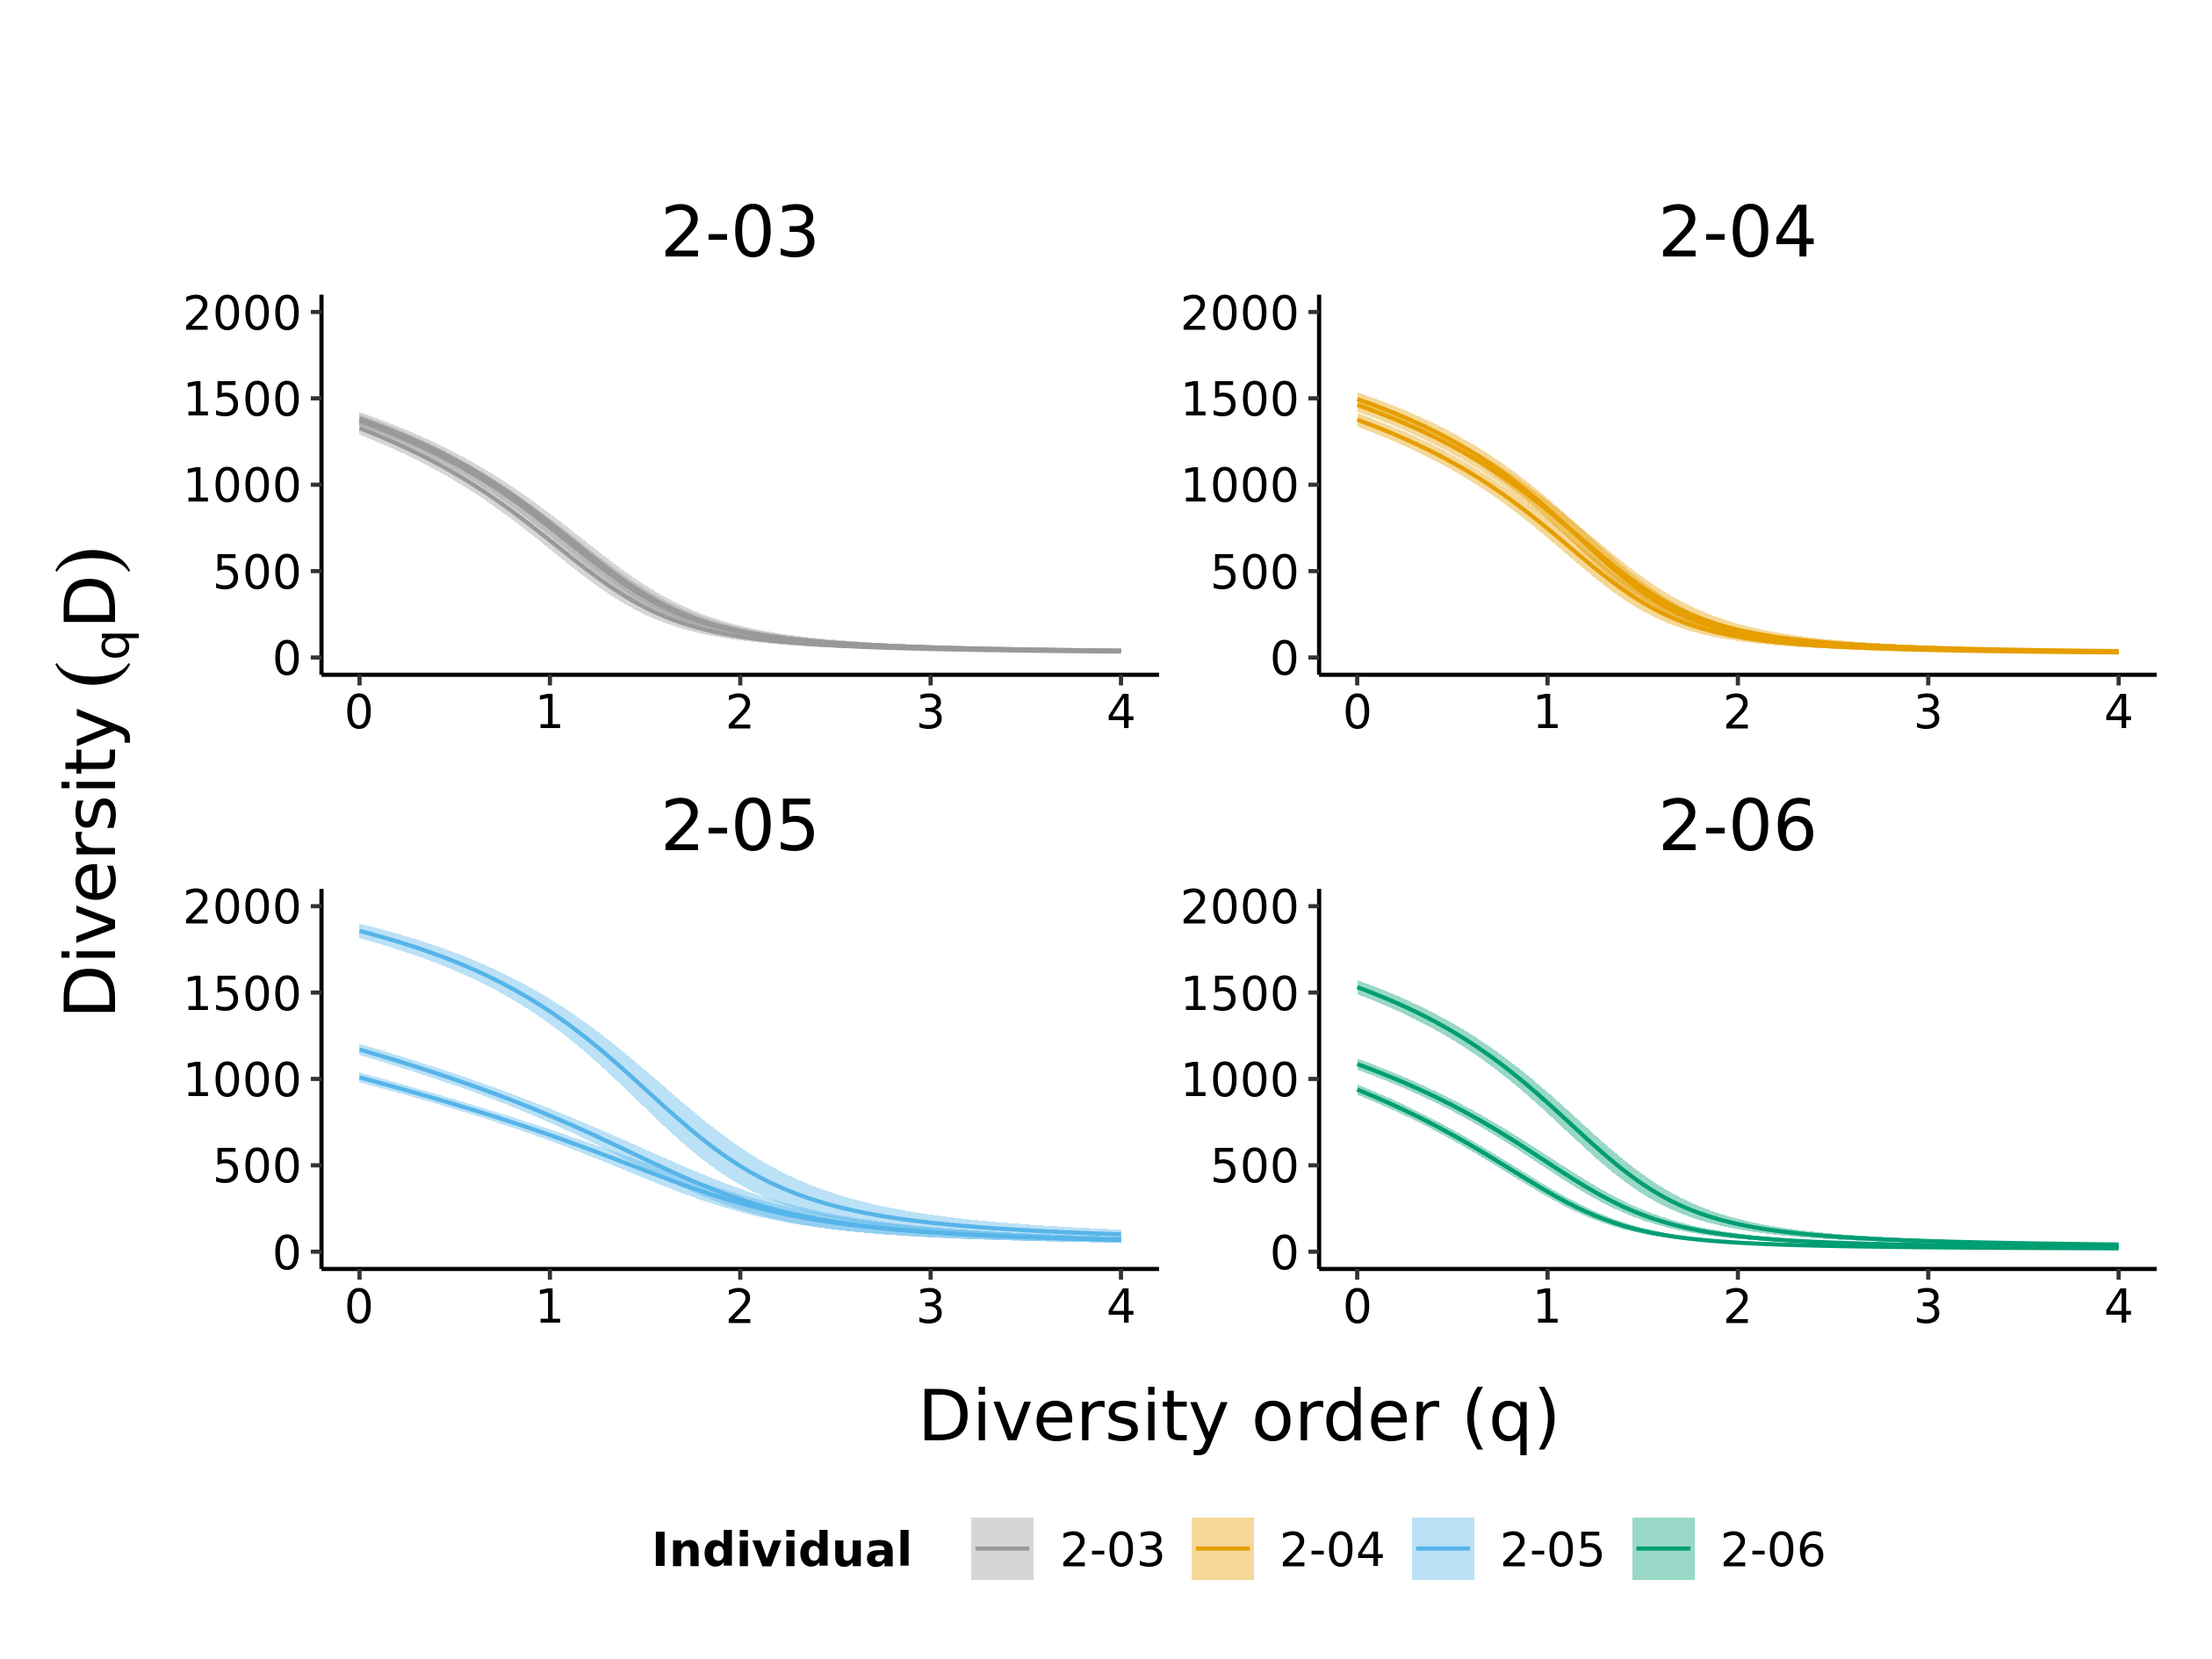
\includegraphics[width = 0.8\textwidth]{_Figures/png/pilot-clone-diversity-solo-spectra}
\caption[Per-replicate clonal diversity spectra for pilot dataset]{\textbf{Per-replicate clonal diversity spectra for pilot dataset:} Hill diversity spectra of clone sizes (as measured by number of unique sequences per clone) for each replicate in the \igseq pilot dataset, grouped by source individual.}
\label{fig:igseq-pilot-clone-diversity-solo-spectra}
\end{figure}

\begin{figure}
\centering
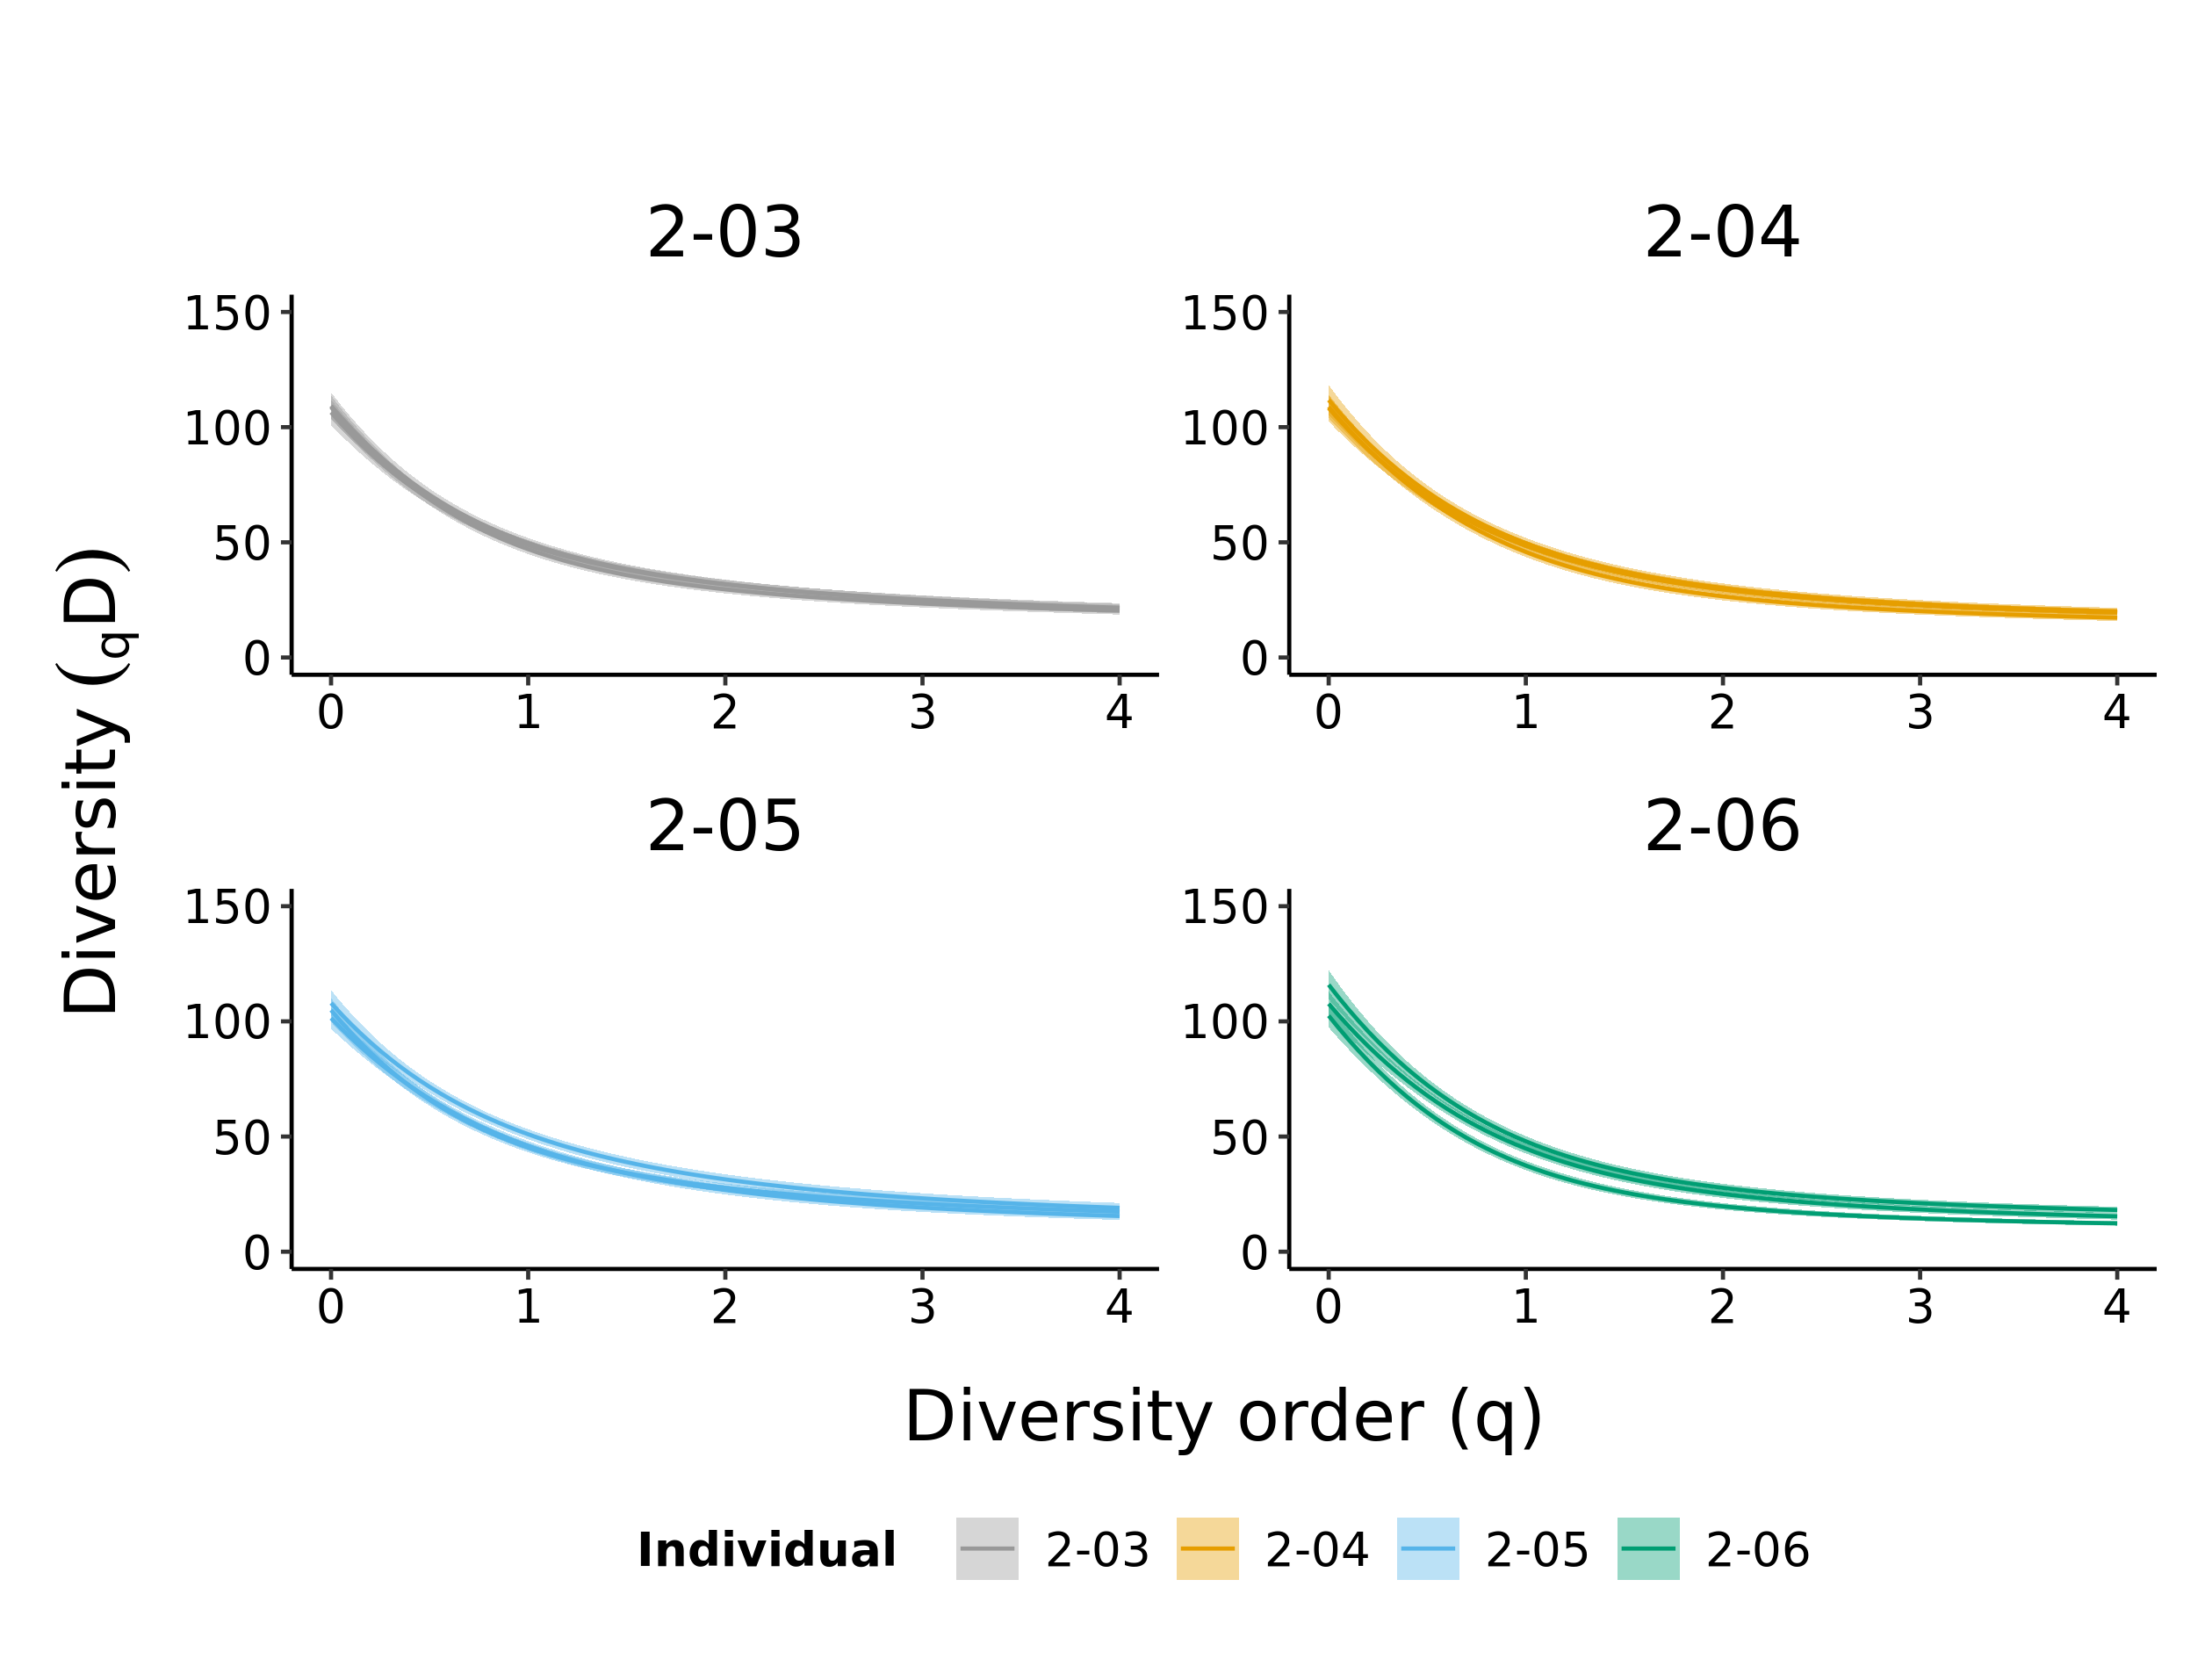
\includegraphics[width = 0.8\textwidth]{_Figures/png/pilot-vj-diversity-solo-spectra}
\caption[Per-replicate VJ-diversity spectra for pilot dataset]{\textbf{Per-replicate VJ-diversity spectra for pilot dataset:} Hill diversity spectra of VJ usage (as measured by number of unique sequences per V/J combination) for each replicate in the \igseq pilot dataset, grouped by source individual.}
\label{fig:igseq-pilot-vj-diversity-solo-spectra}
\end{figure}

\begin{figure}
\centering
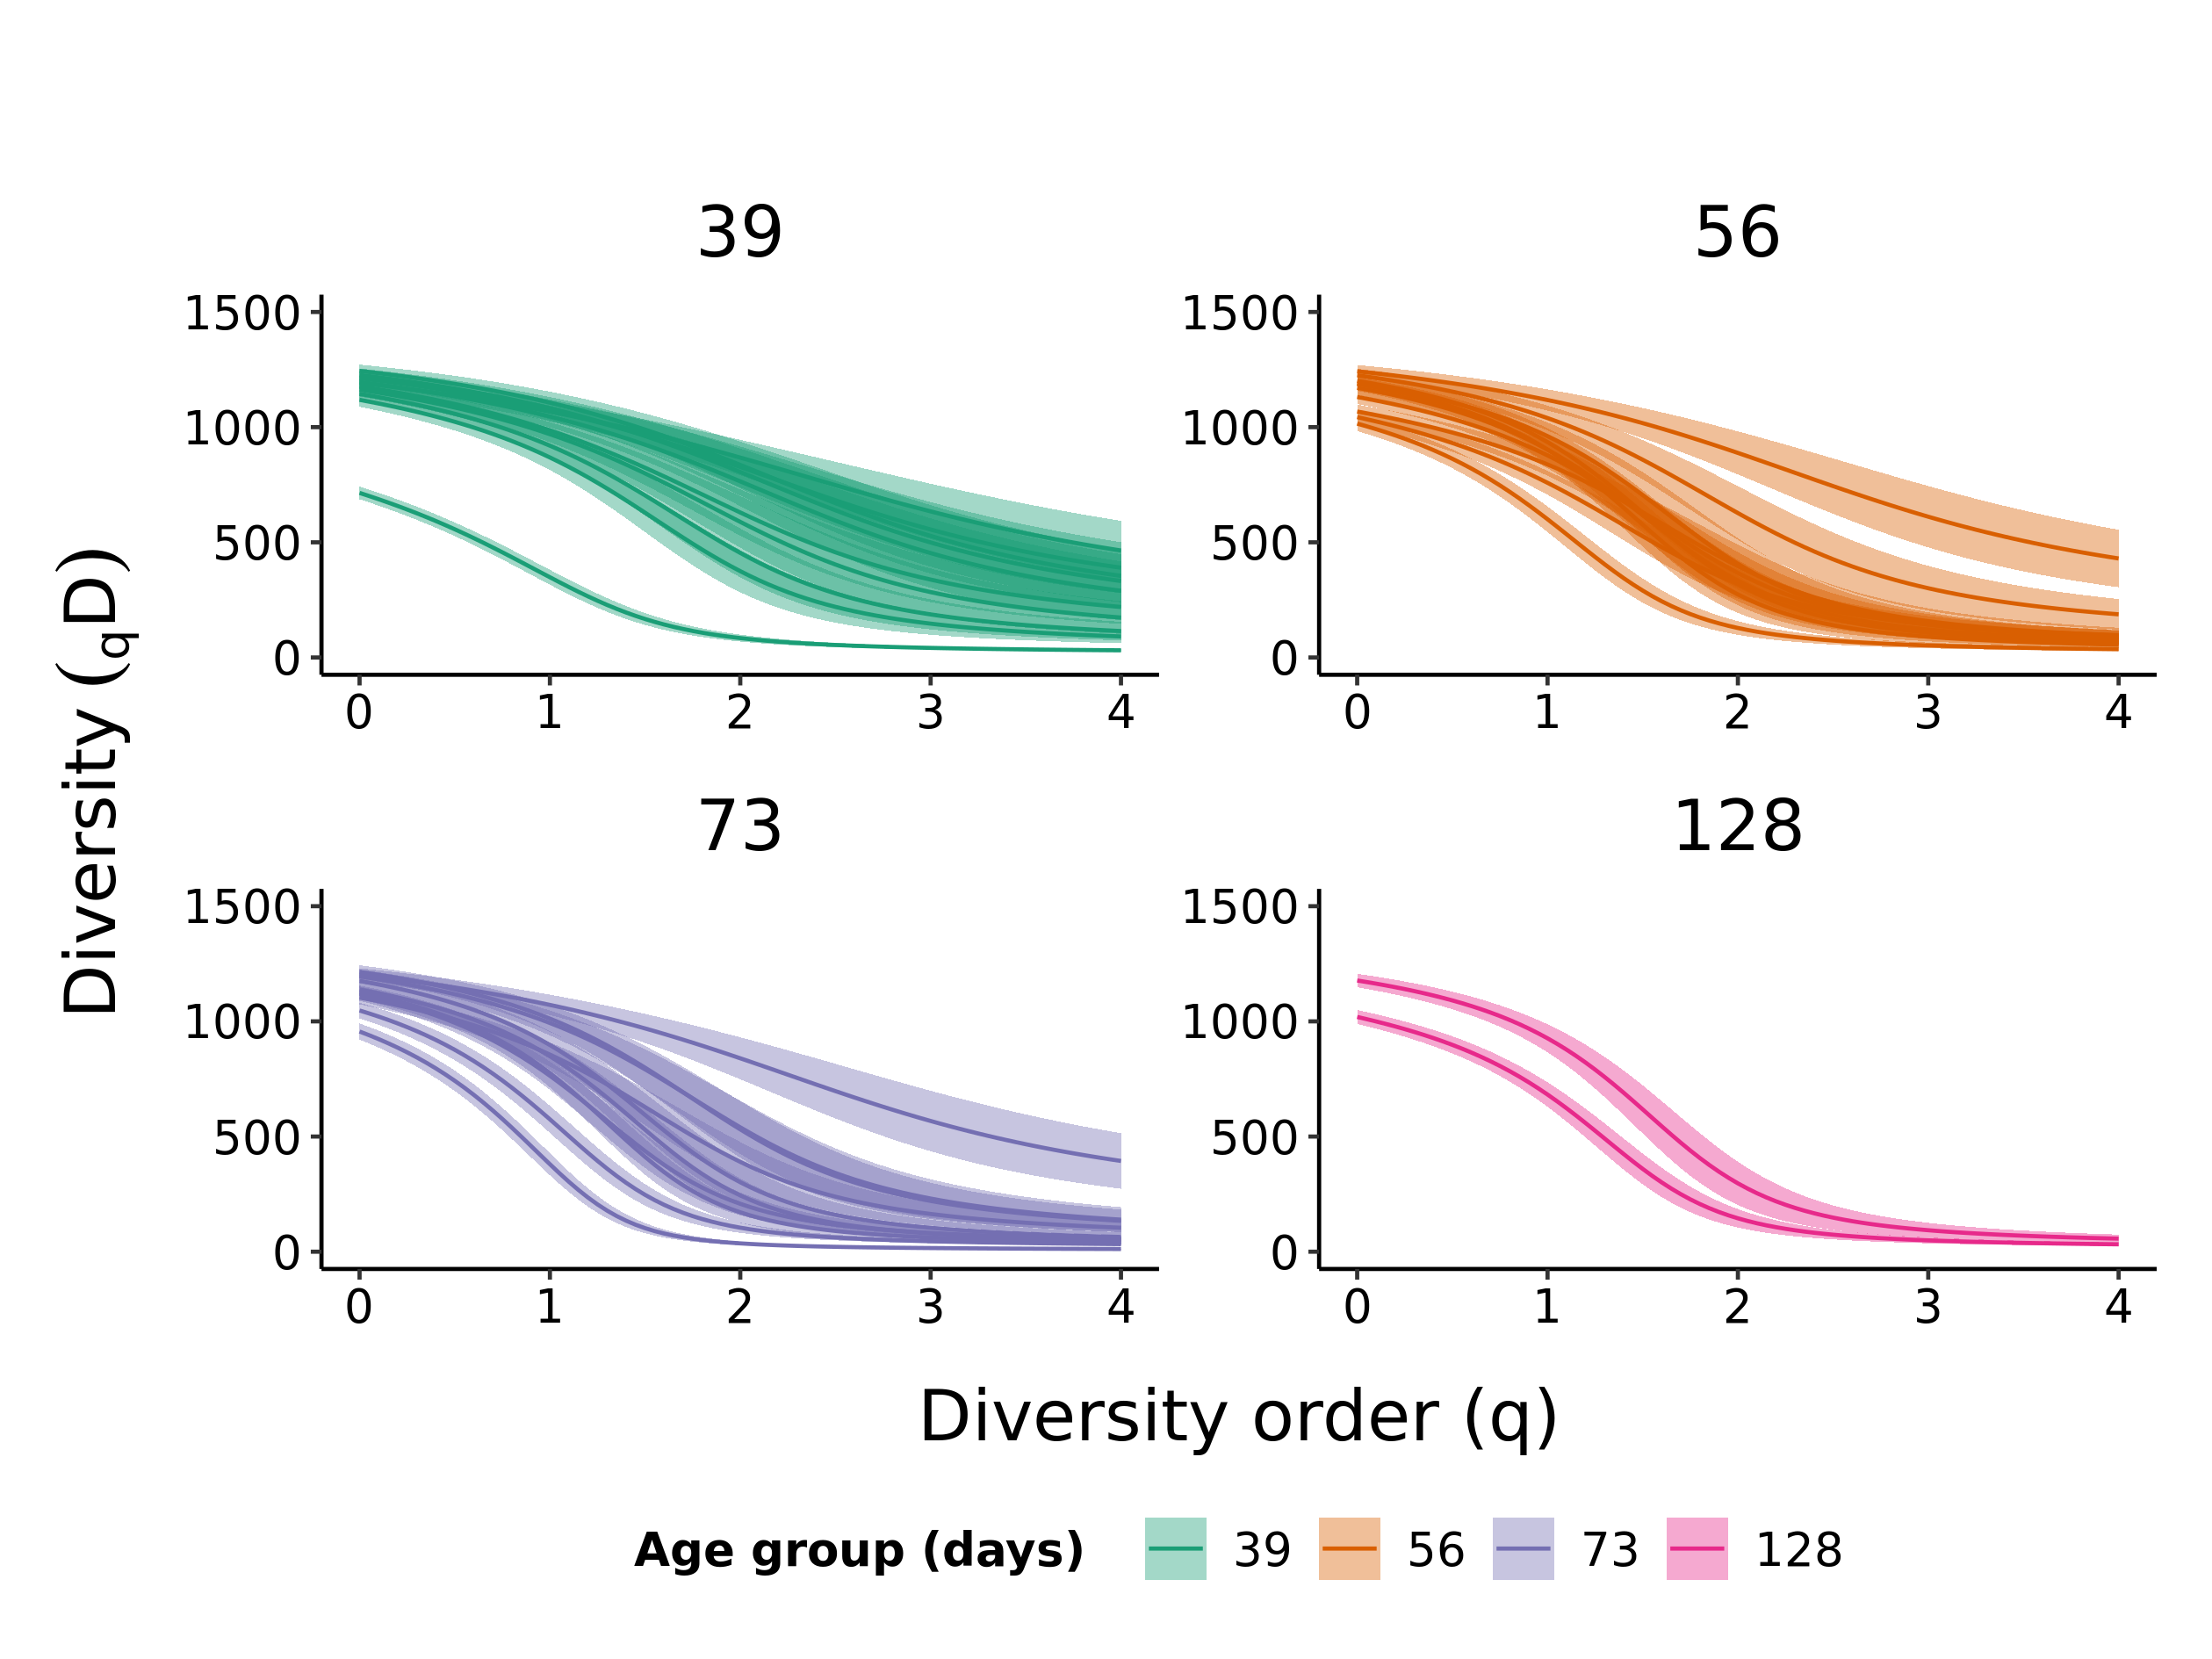
\includegraphics[width = 0.8\textwidth]{_Figures/png/ageing-clone-diversity-solo-spectra}
\caption[Per-individual clonal diversity spectra for ageing dataset]{\textbf{Per-individual clonal diversity spectra for ageing dataset:} Hill diversity spectra of clone sizes (as measured by number of unique sequences per clone) for each individual in the \igseq pilot dataset, grouped by age at death.}
\label{fig:igseq-ageing-clone-diversity-solo-spectra}
\end{figure}

\begin{figure}
\centering
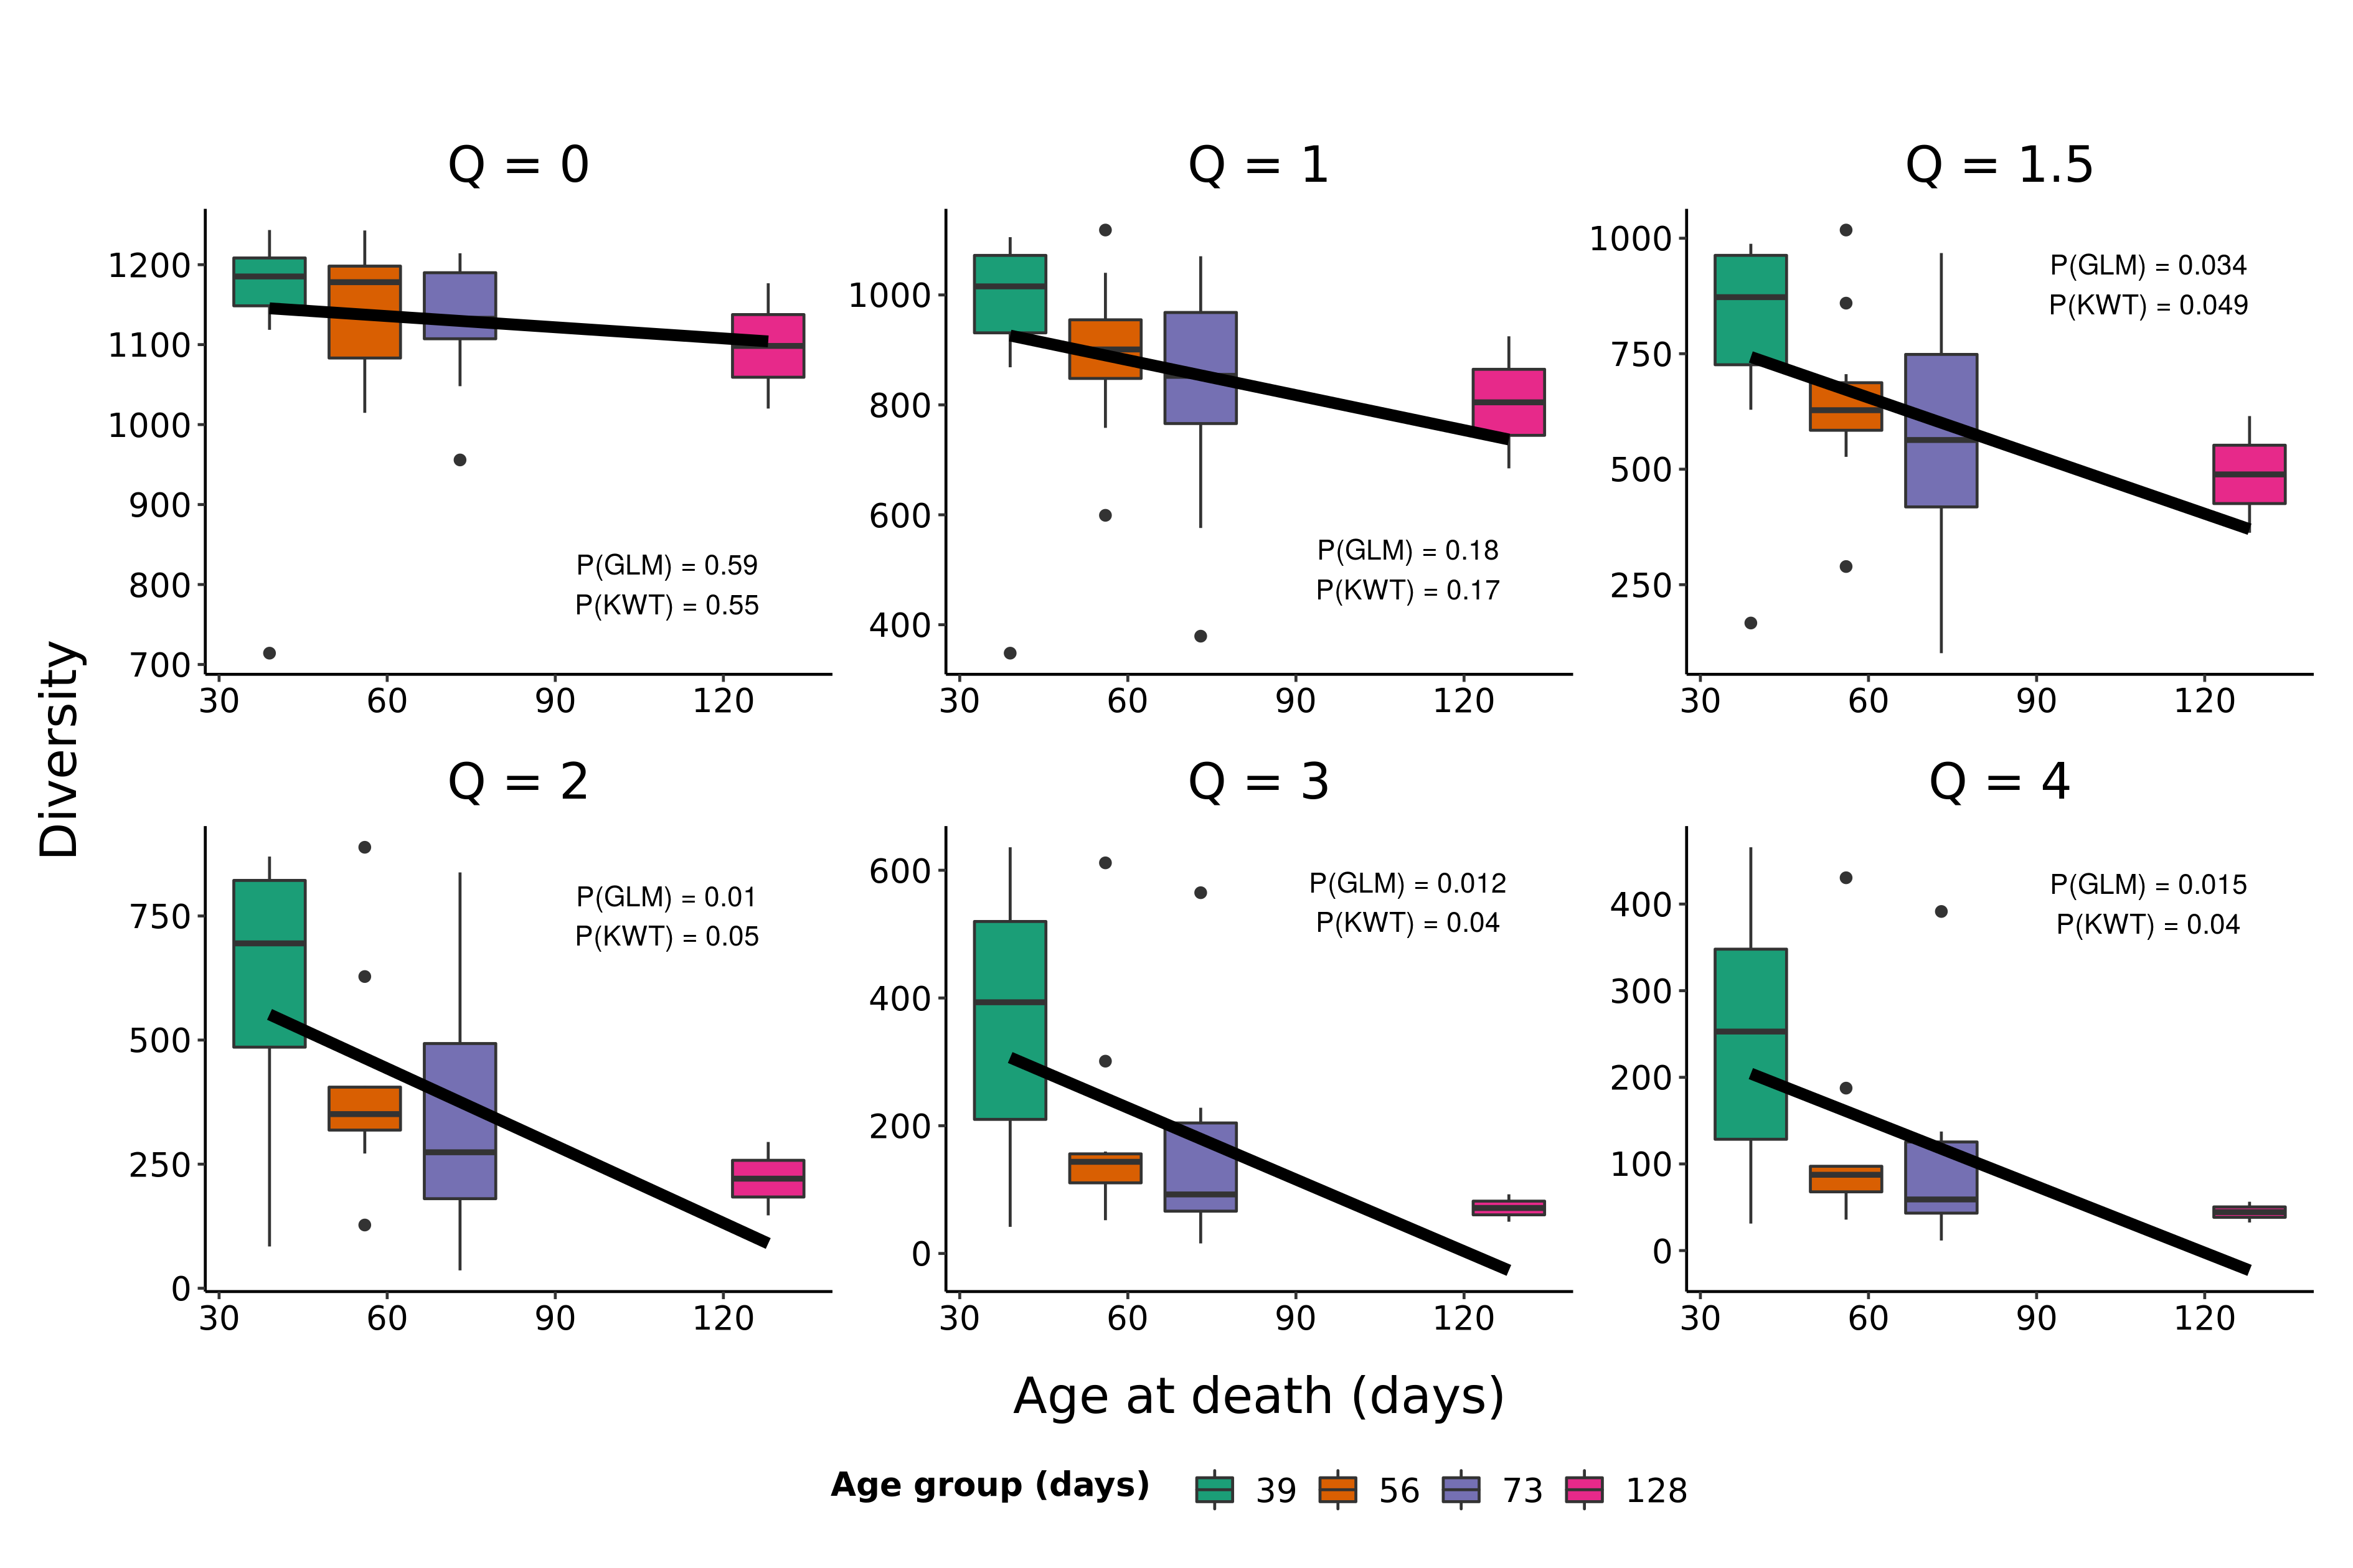
\includegraphics[width = 0.8\textwidth]{_Figures/png/ageing-clone-diversity-solo-fit-linear}
\caption[Comparing clonal alpha-diversities between age groups in the \igseq ageing dataset (linear fit)]{\textbf{Comparing clonal alpha-diversities between age groups in the \igseq ageing dataset (linear fit):} Boxplots of Hill diversity values for the antibody repertoires of individuals of each age group in the \igseq ageing dataset at a sample of diversity orders, overlaid with the predictions of the best-fit linear model at each order.  Annotated $p$-values indicate the statistical significance of the estimated age effect on diversity under the linear model ($P(GLM)$) and a Kruskal-Wallis test ($P(KWT)$) for each diversity order.}
\label{fig:igseq-ageing-clone-diversity-solo-fit-linear}
\end{figure}

\begin{figure}
\centering
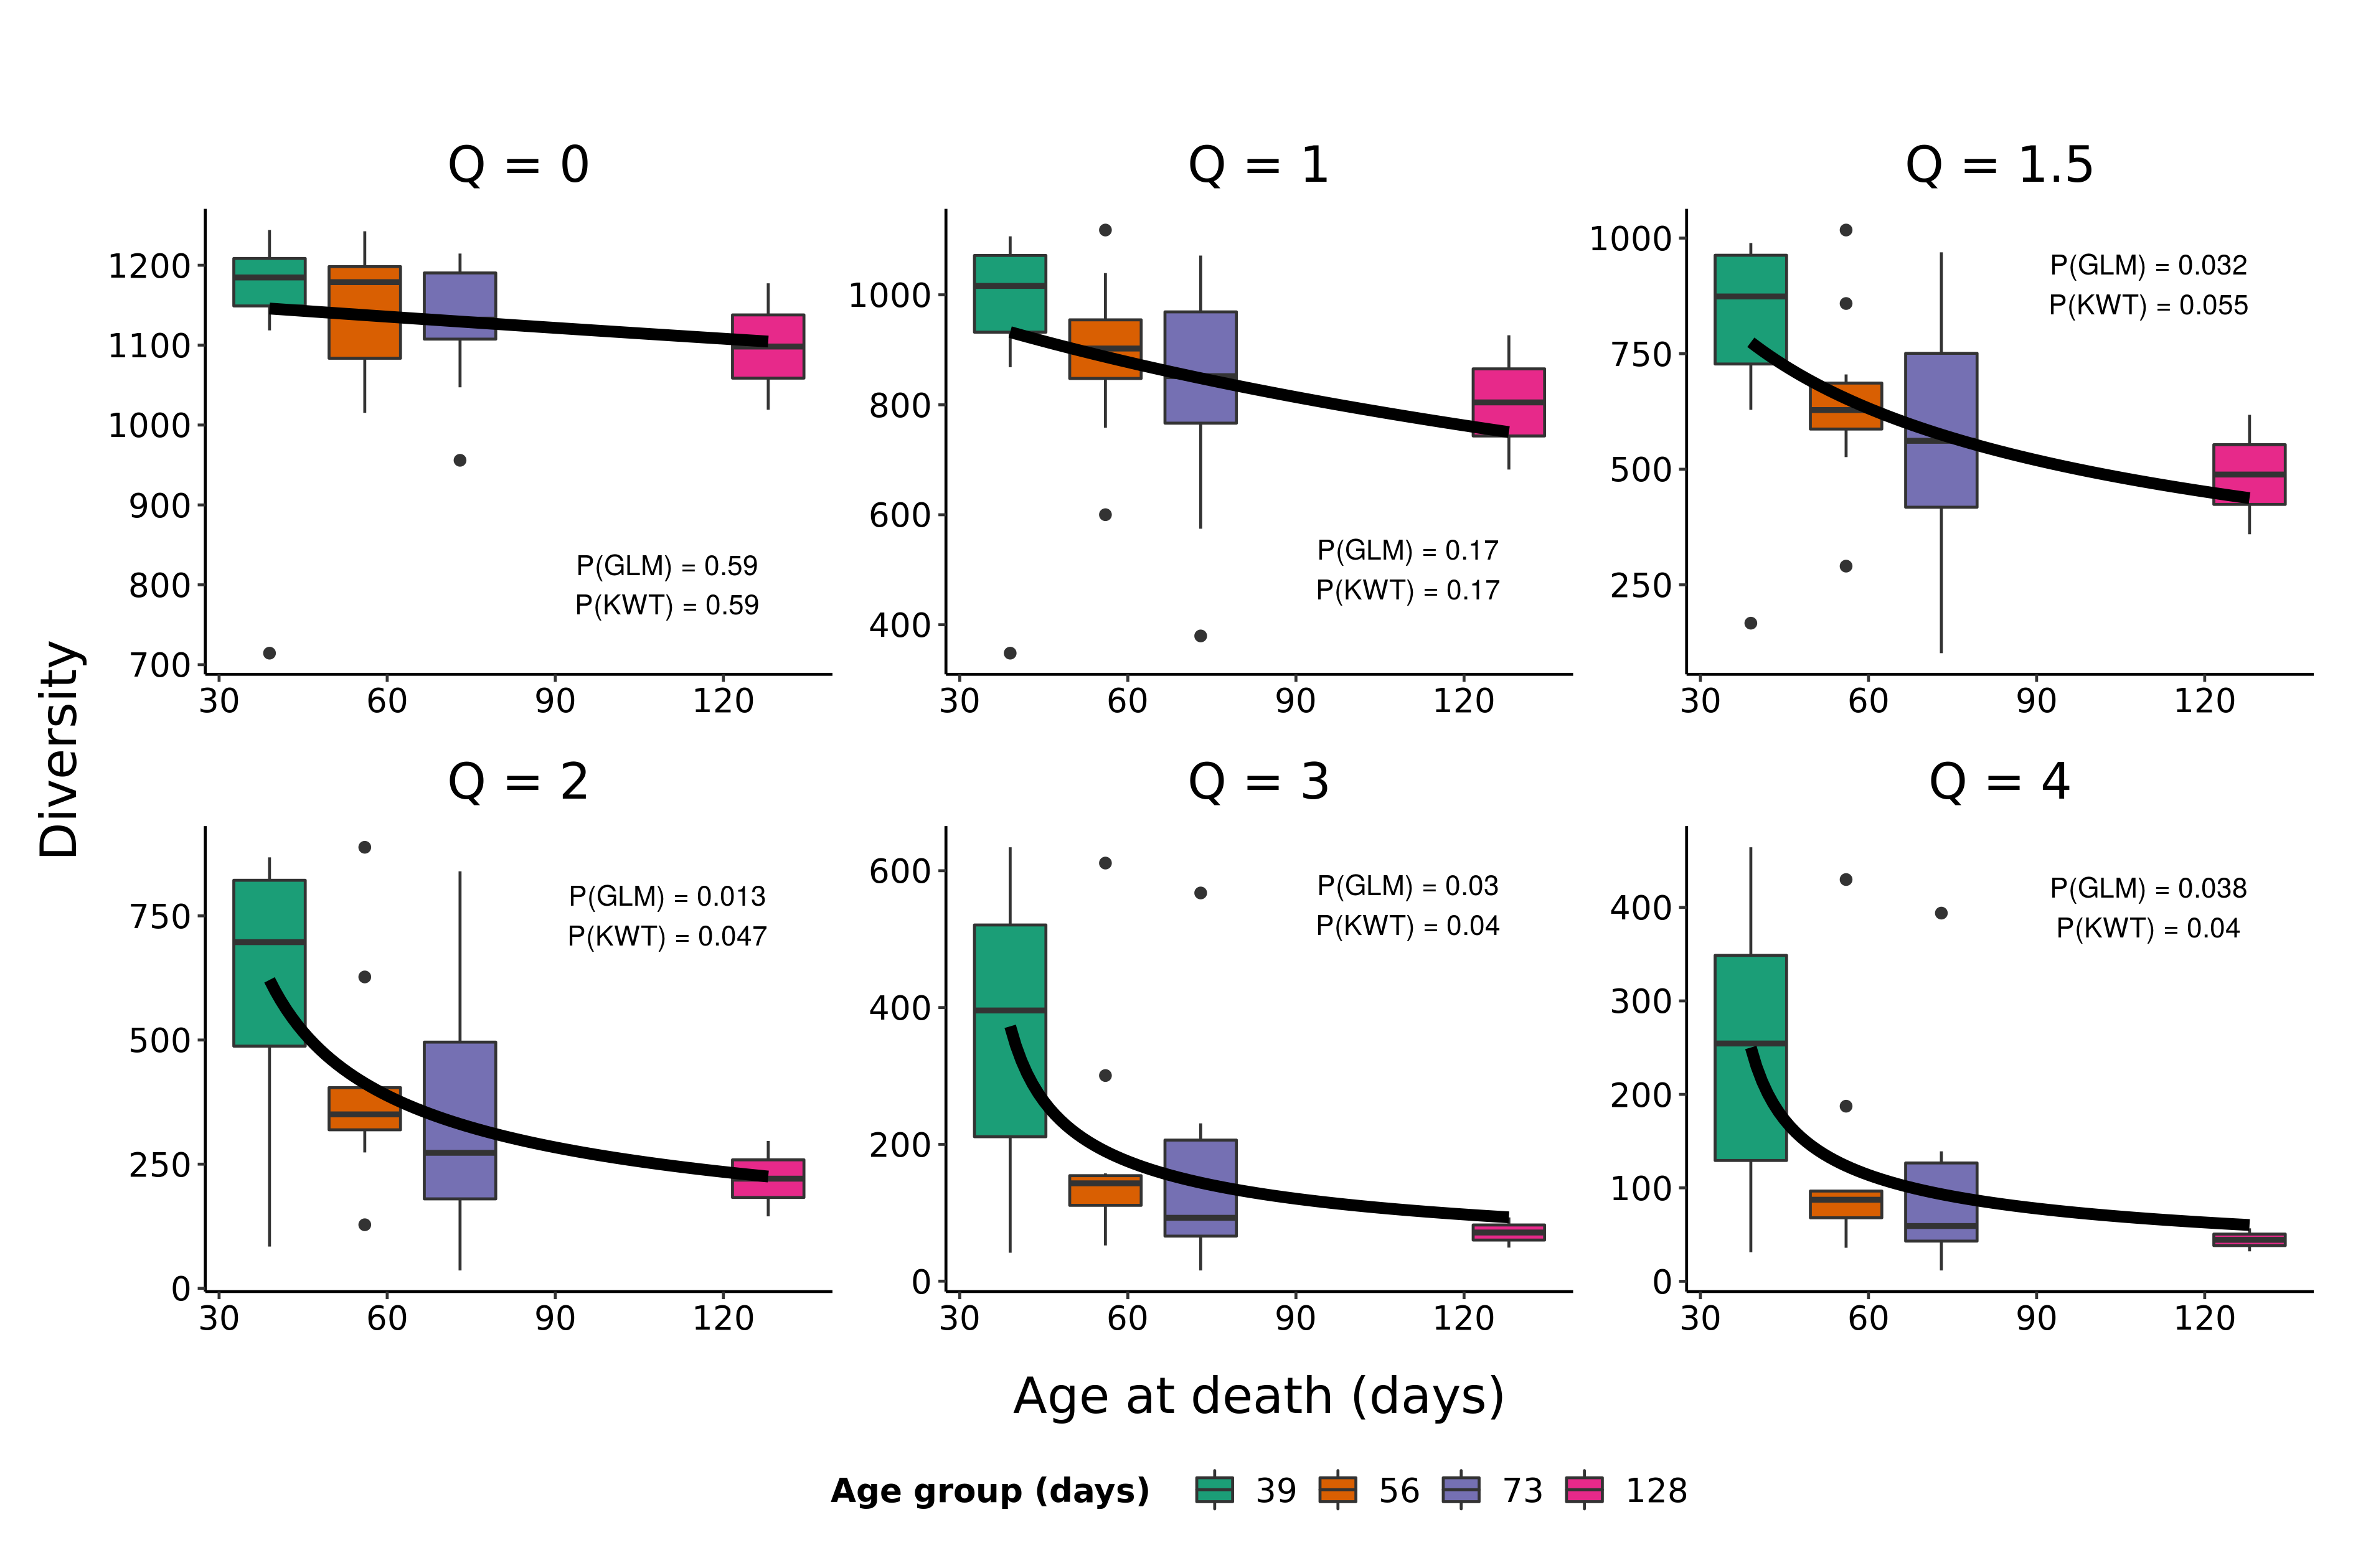
\includegraphics[width = 0.8\textwidth]{_Figures/png/ageing-clone-diversity-solo-fit-igauss}
\caption[Comparing clonal alpha-diversities between age groups in the \igseq ageing dataset (inverse-Gaussian fit)]{\textbf{Comparing clonal alpha-diversities between age groups in the \igseq ageing dataset (inverse-Gaussian fit):} Boxplots of Hill diversity values for the antibody repertoires of individuals of each age group in the \igseq ageing dataset at a sample of diversity orders, overlaid with the predictions of the best-fit inverse-Gaussian-distributed generalised linear model at each order.  Annotated $p$-values indicate the statistical significance of the estimated age effect on diversity under the GLM ($P(GLM)$) and a Kruskal-Wallis test ($P(KWT)$) for each diversity order.}
\label{fig:igseq-ageing-clone-diversity-solo-fit-igauss}
\end{figure}

\begin{figure}
\centering
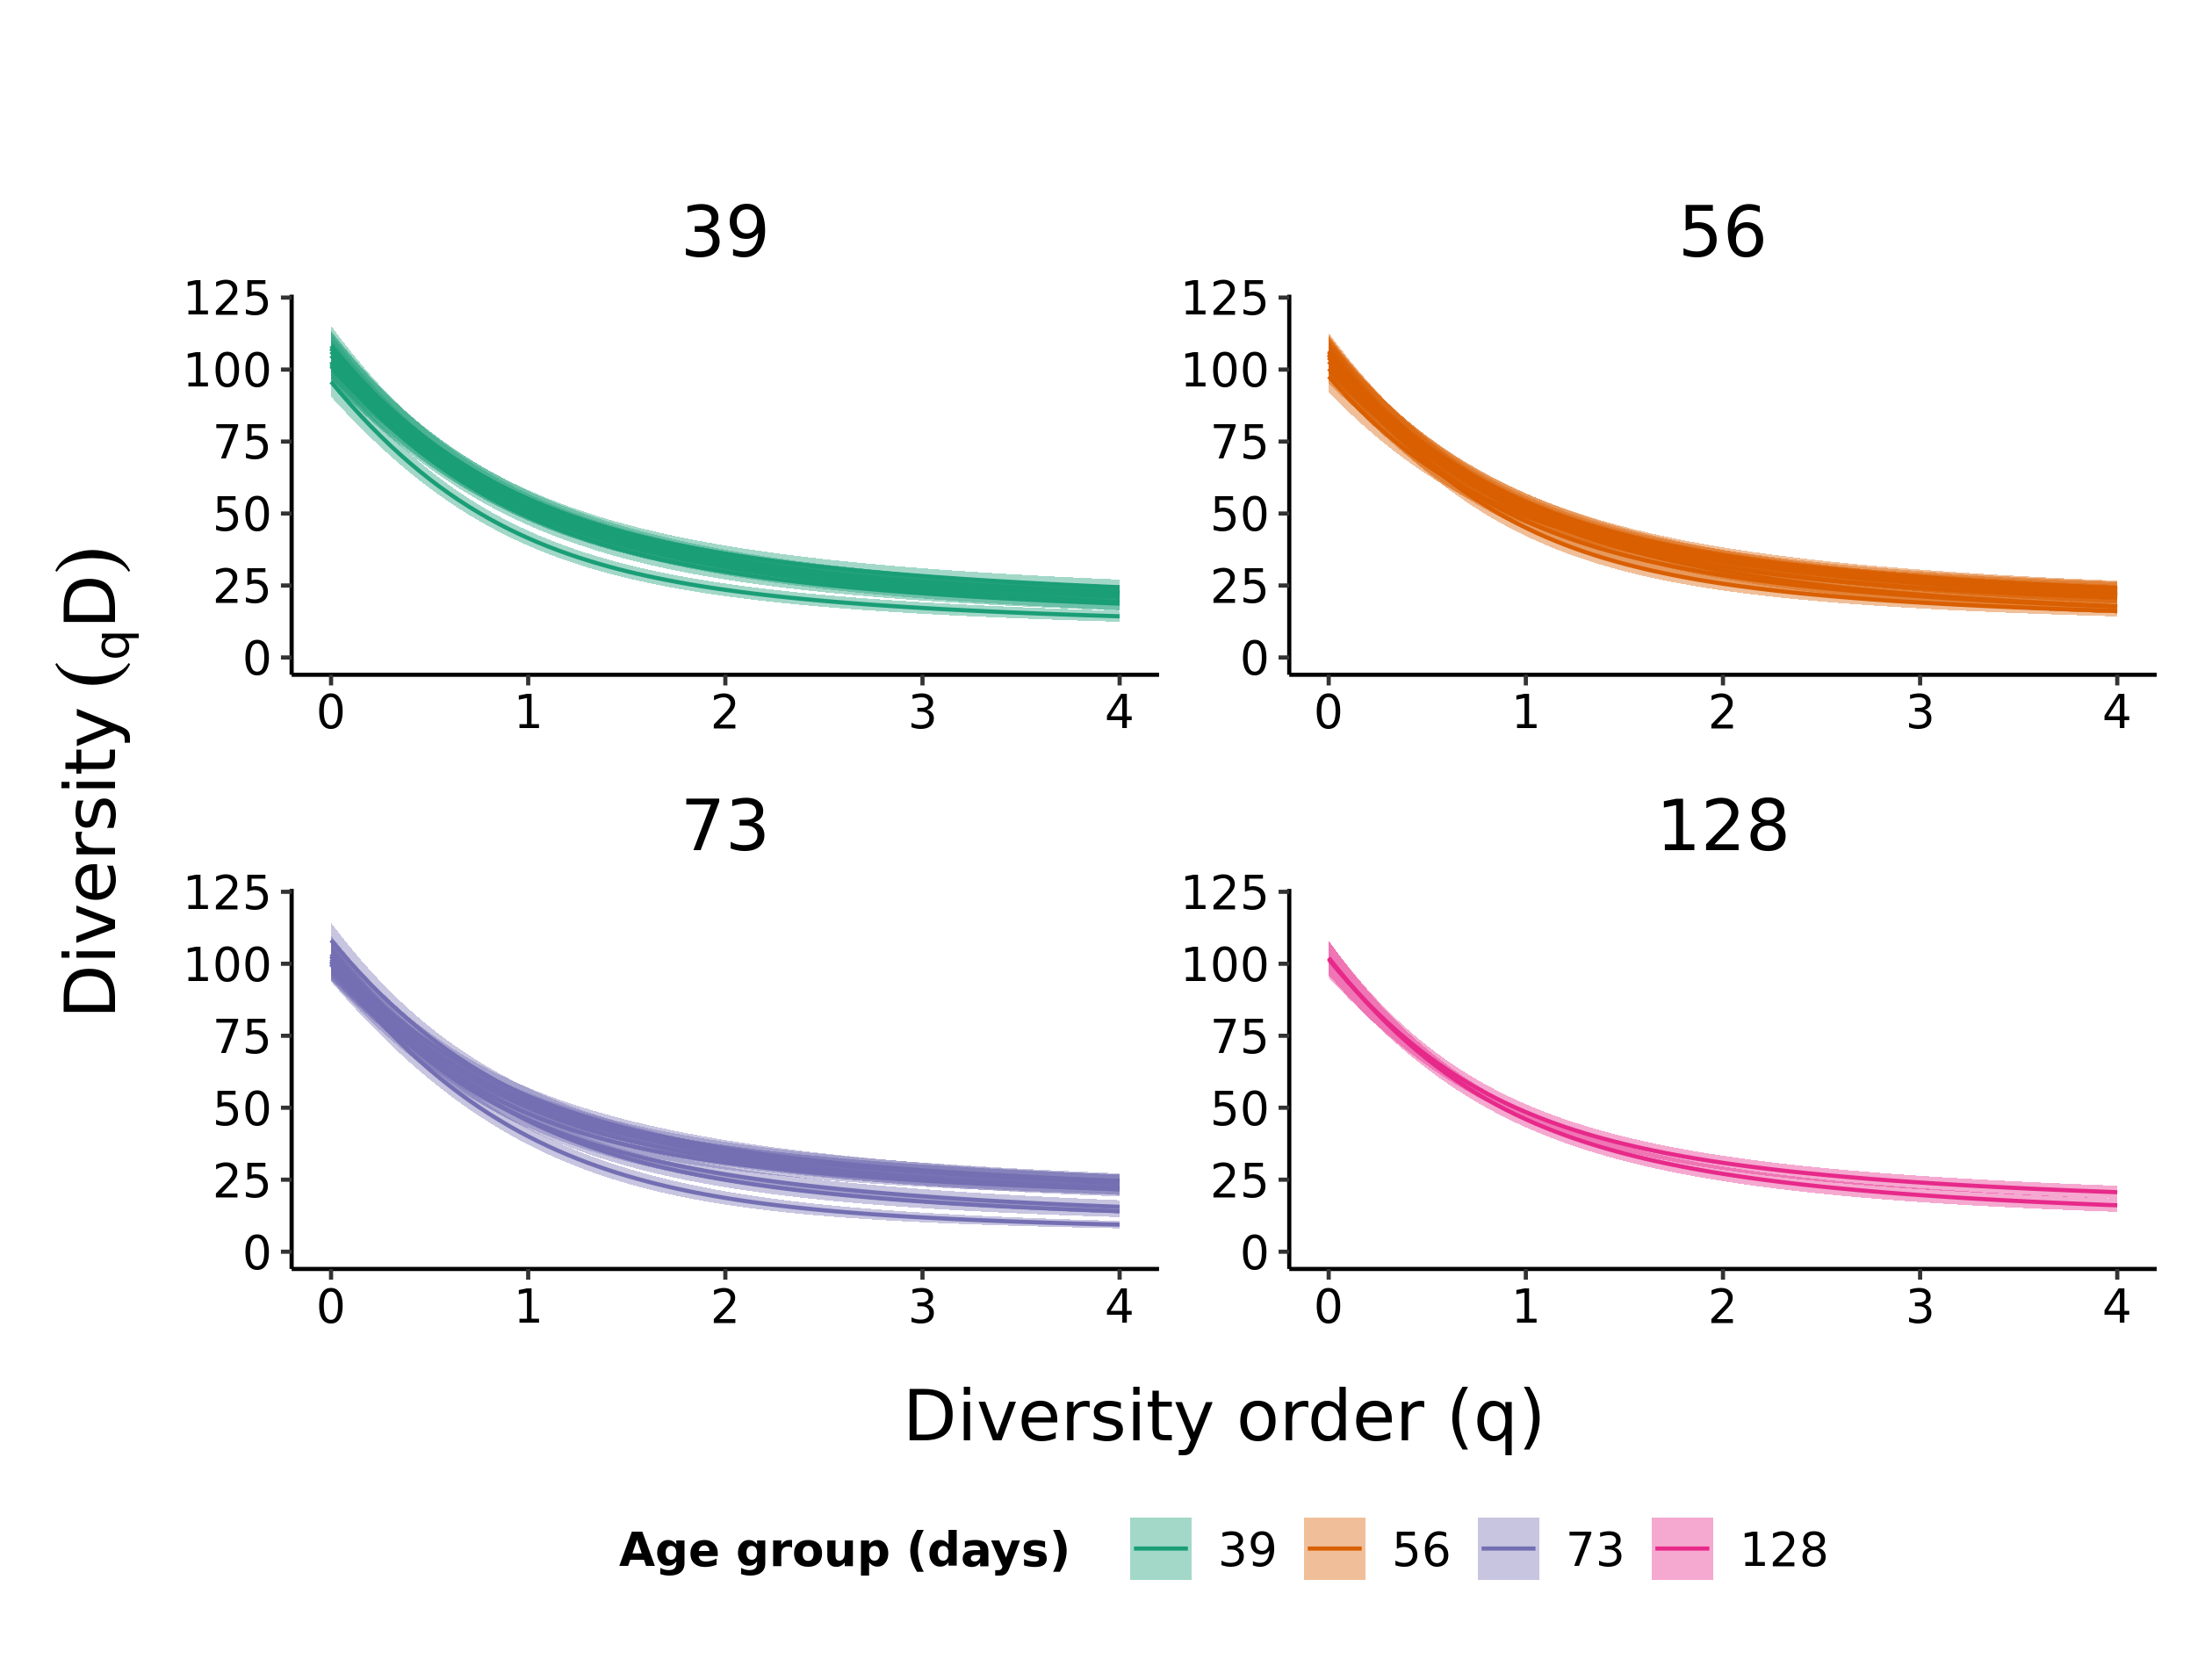
\includegraphics[width = 0.8\textwidth]{_Figures/png/ageing-VJ-diversity-solo-spectra}
\caption[Per-individual clonal diversity spectra for ageing dataset]{\textbf{Per-individual clonal diversity spectra for ageing dataset:} Hill diversity spectra of VJ usage (as measured by number of unique sequences per V/J combination) for each individual in the \igseq pilot dataset, grouped by age at death.}
\label{fig:igseq-ageing-vj-diversity-solo-spectra}
\end{figure}

\begin{figure}
\centering
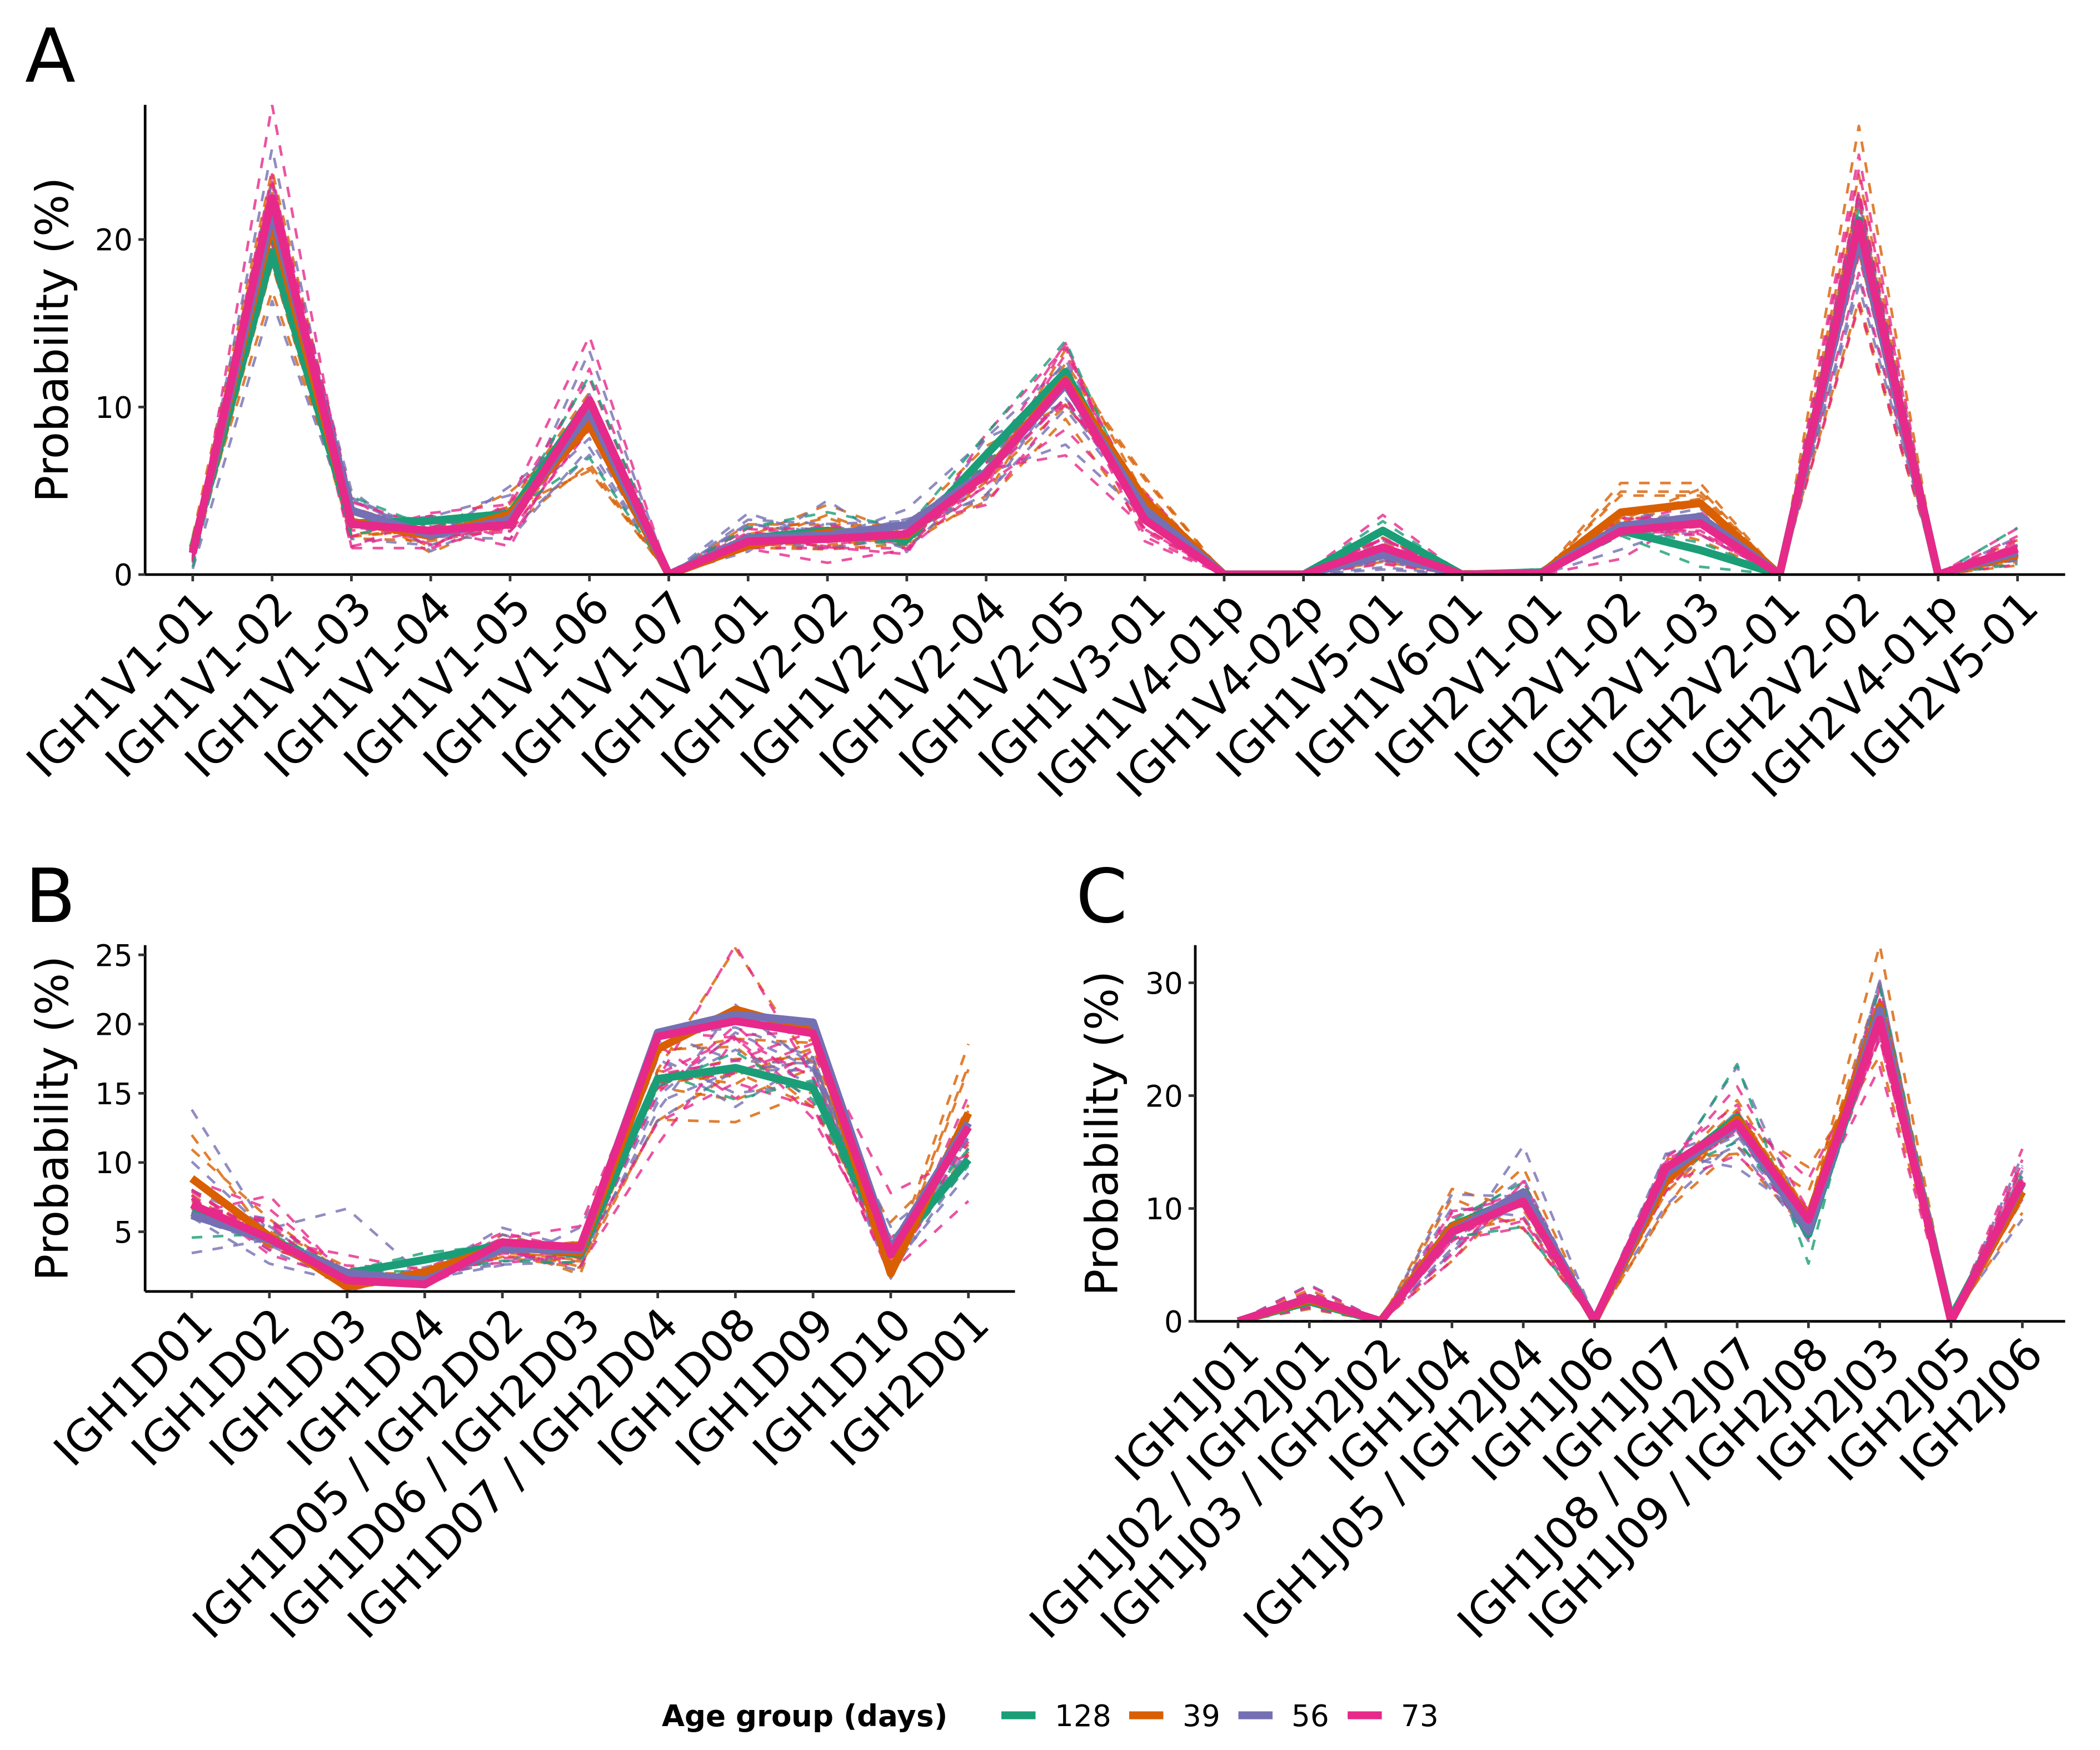
\includegraphics[width = 0.8\textwidth]{_Figures/png/ageing-igor-segments}
\caption[Segment-choice distributions during primary diversification in the ageing dataset]
{\textbf{Segment-choice distributions during primary diversification in the ageing dataset:} Probability distributions of segment choice for (A) \vh-, (B) \dh- and (C) \jh-segments during VDJ recombination in adult male turquoise killifish of different ages, inferred from the \igseq ageing dataset using \program{IGoR}. Thin dashed lines represent the distributions inferred for individual killifish, while the thick solid lines represents those inferred from pooled data from all individuals in each age group. \dh and \jh segments with identical sequences (which cannot be distinguished in the repertoire data even in principle) are collapsed together.}
\label{fig:igseq-ageing-igor-segments}
\end{figure}

\begin{figure}
\centering
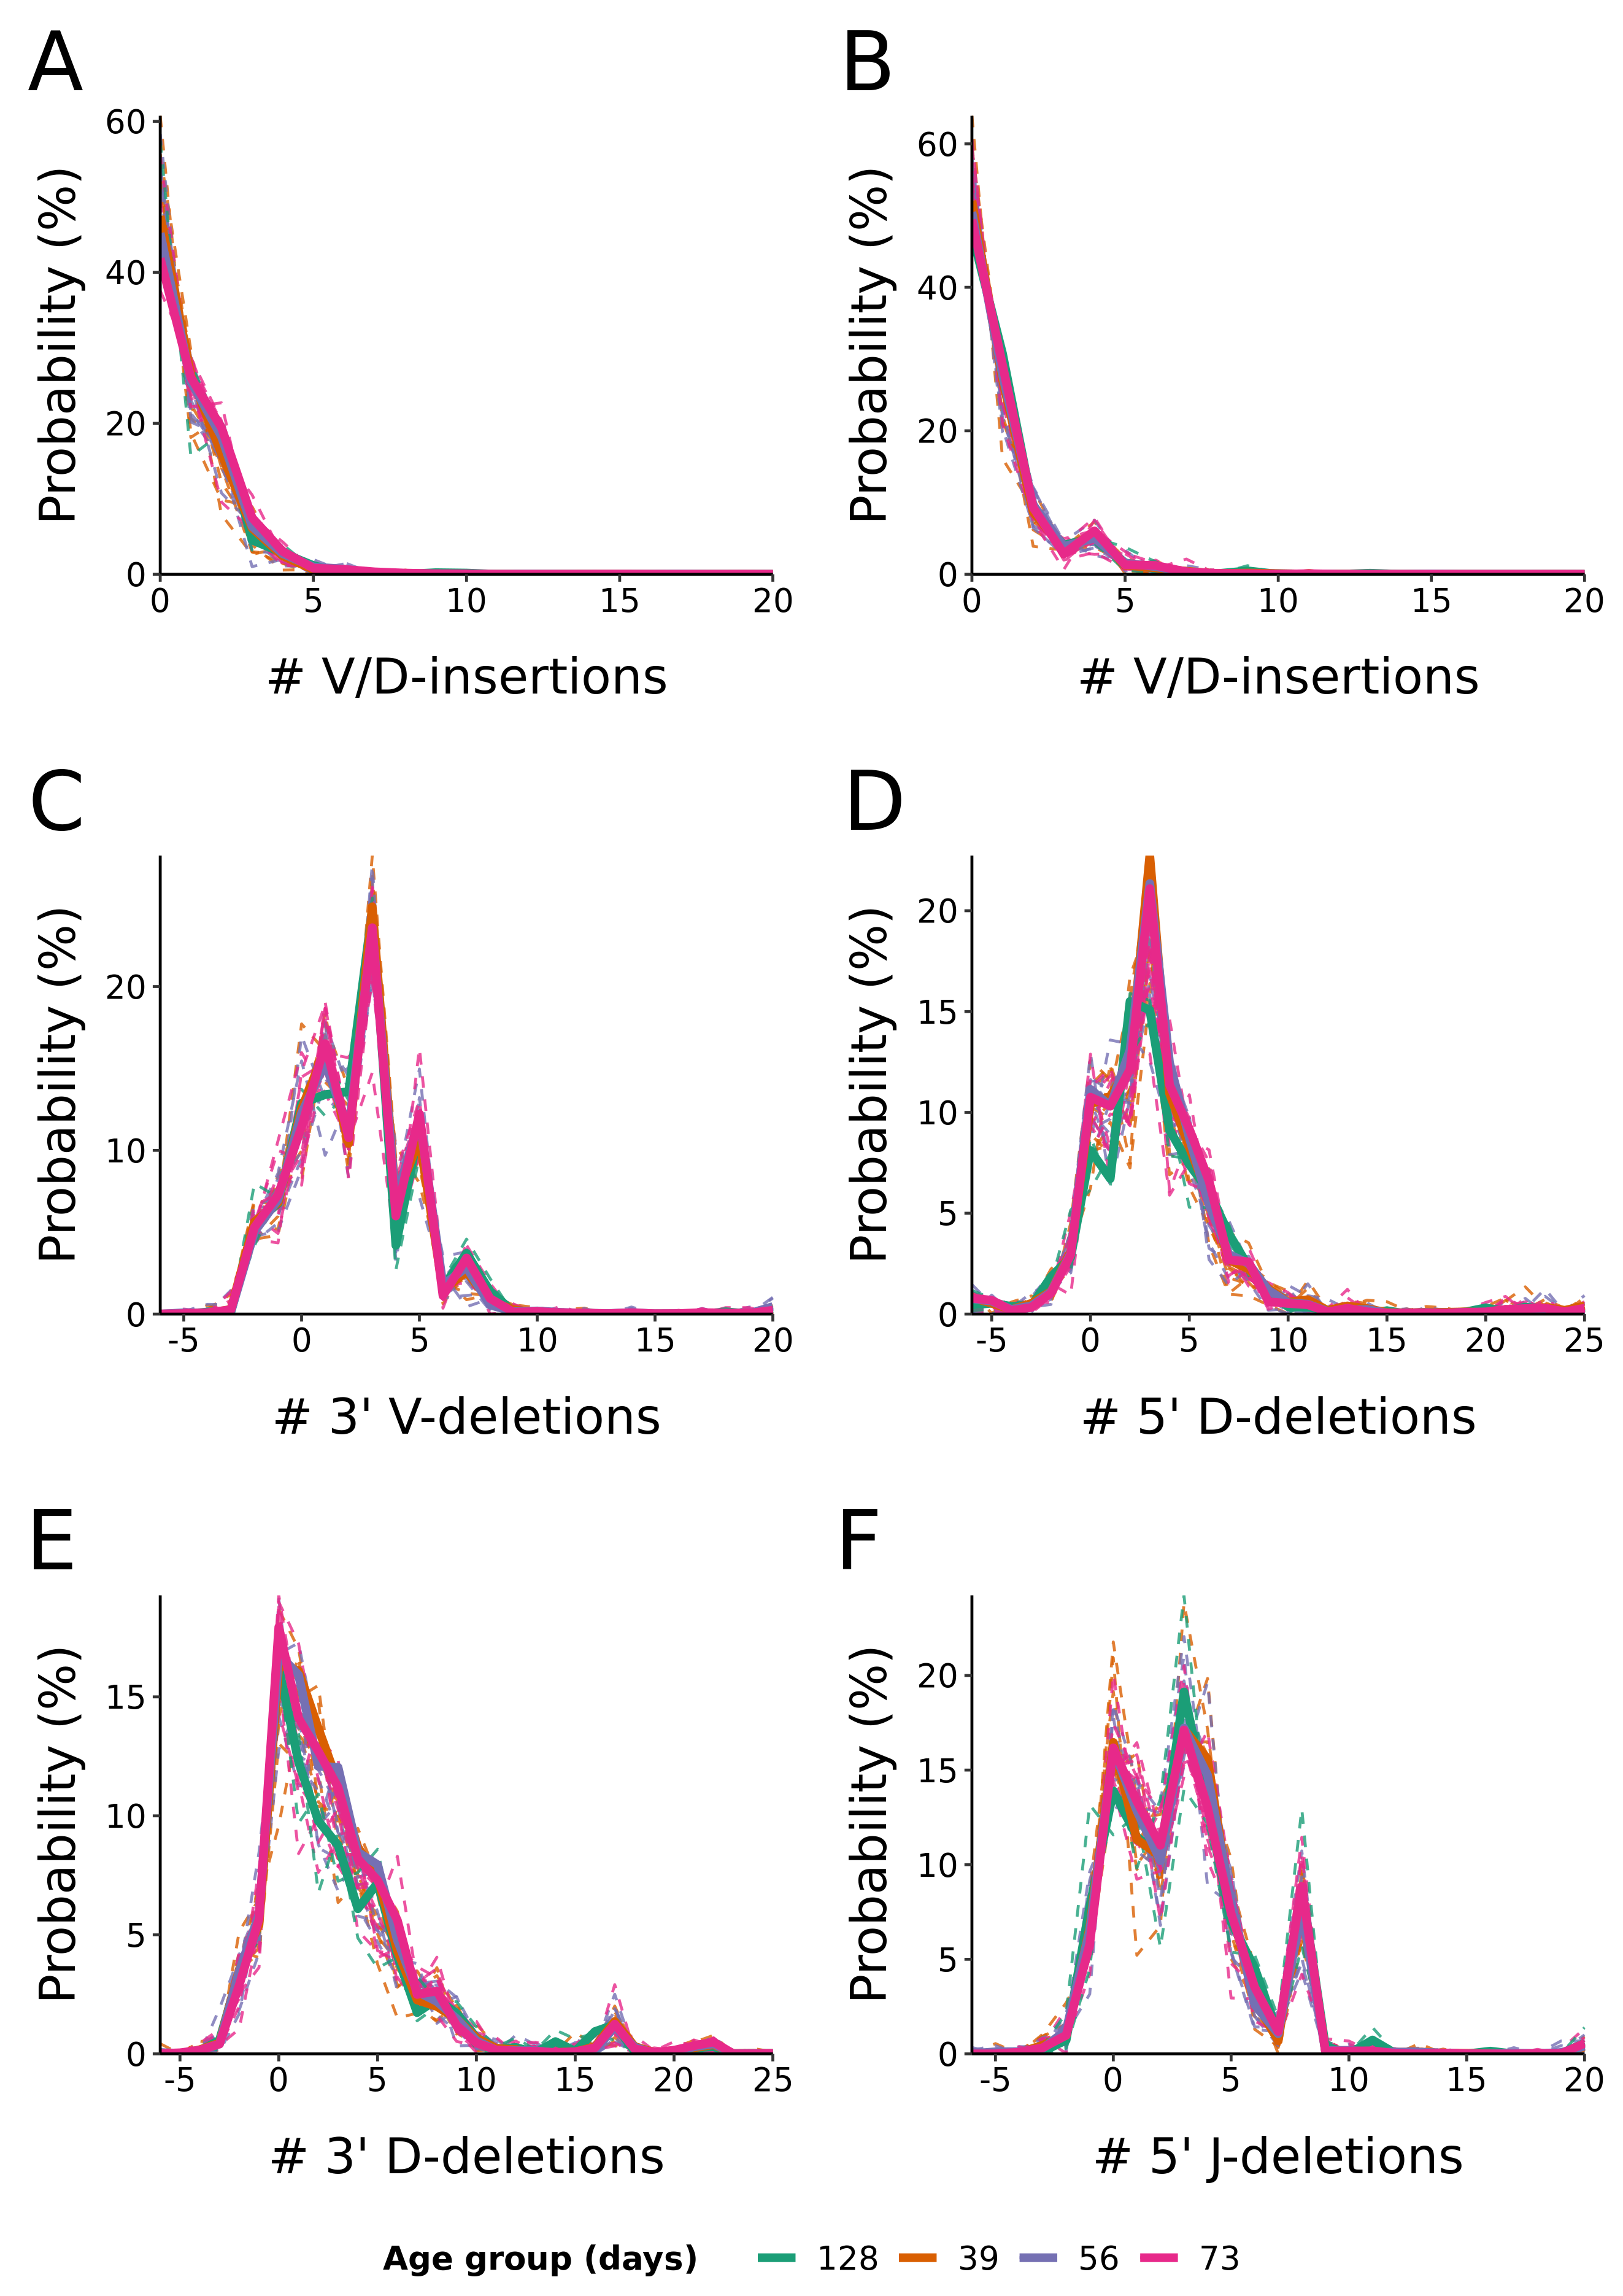
\includegraphics[width = 0.8\textwidth]{_Figures/png/ageing-igor-indels}
\begin{subfigure}{0em}
\phantomsubcaption{}
\label{fig:igseq-ageing-igor-indels-vdins}
\end{subfigure}
\begin{subfigure}{0em}
\phantomsubcaption{}
\label{fig:igseq-ageing-igor-indels-djins}
\end{subfigure}
\begin{subfigure}{0em}
\phantomsubcaption{}
\label{fig:igseq-ageing-igor-indels-vdel}
\end{subfigure}
\begin{subfigure}{0em}
\phantomsubcaption{}
\label{fig:igseq-ageing-igor-indels-d5del}
\end{subfigure}
\begin{subfigure}{0em}
\phantomsubcaption{}
\label{fig:igseq-ageing-igor-indels-d3del}
\end{subfigure}
\begin{subfigure}{0em}
\phantomsubcaption{}
\label{fig:igseq-ageing-igor-indels-jdel}
\end{subfigure}
\caption[Insertion/deletion distributions during primary diversification in the ageing dataset]
{\textbf{Insertion/deletion distributions during primary diversification in the ageing dataset:} Probability distributions of the number of N-insertions (A-B) or P-insertions/deletions (C-F) following VDJ recombination in adult male turquoise killifish of different ages, inferred from the \igseq ageing dataset using \program{IGoR}. P-insertions are modelled as negative deletions. Thin dashed lines represent the distributions inferred for individual killifish, while the thick solid lines represents those inferred from pooled data from all individuals in each age group.}
\label{fig:igseq-ageing-igor-indels}
\end{figure}

\begin{figure}
\centering
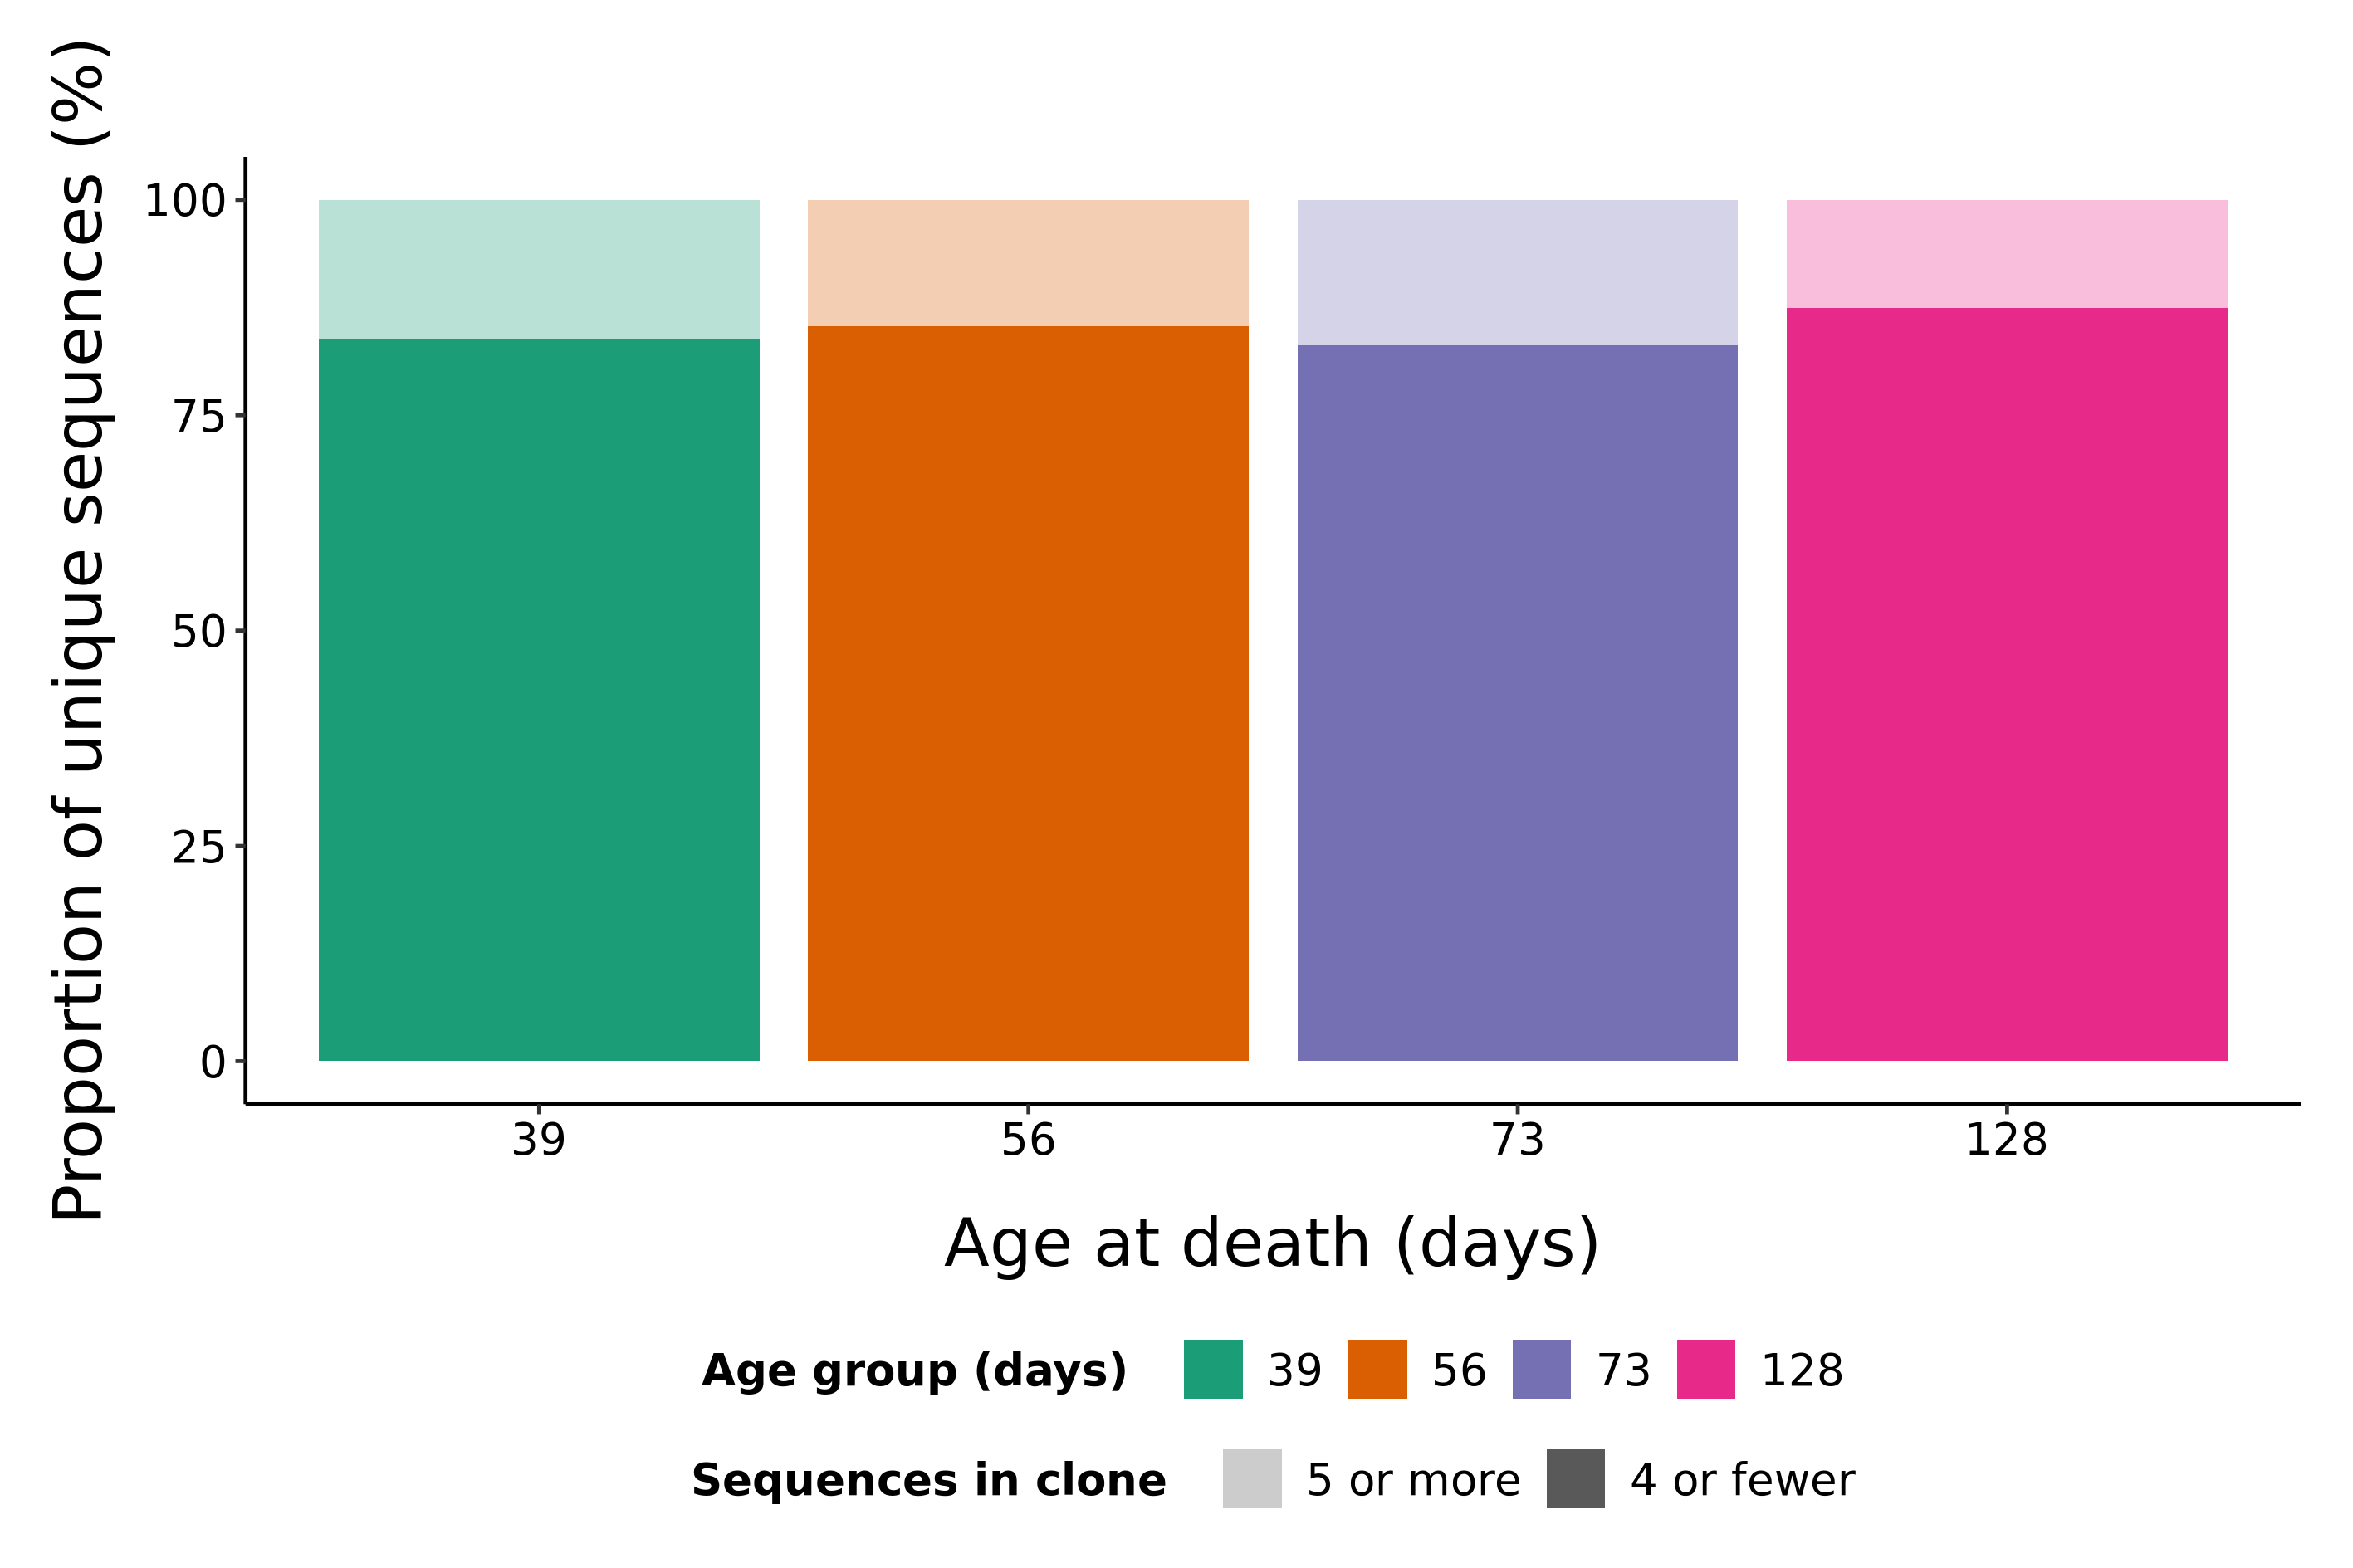
\includegraphics[width = 0.9\textwidth]{_Figures/png/ageing-pc-seq-in-small-clones}
\caption[Proportion of unique sequences in small clones in the \igseq ageing dataset]{\textbf{Proportion of unique sequences in small clones in the \igseq ageing dataset:} Stacked barplots of average proportion of abundant (5 or more unique sequences, top, pale) vs non-abundant (4 or fewer, bottom, dark) in each age group in the \igseq ageing dataset. The proportion of non-abundant clones does not change significantly with age (Kruskal-Wallis analysis of variance, $p=\embed{_Figures/txt/ageing-pc-seq-in-small-clones-kruskal-p.txt}$).}
\label{fig:igseq-ageing-pc-seq-in-small-clones}
\end{figure}

\begin{figure}
\centering
\begin{subfigure}{0em}
\phantomsubcaption{}
\label{fig:igseq-gut-clone-diversity-solo-spectra-age}
\end{subfigure}
\begin{subfigure}{0em}
\phantomsubcaption{}
\label{fig:igseq-gut-clone-diversity-solo-spectra-groups}
\end{subfigure}
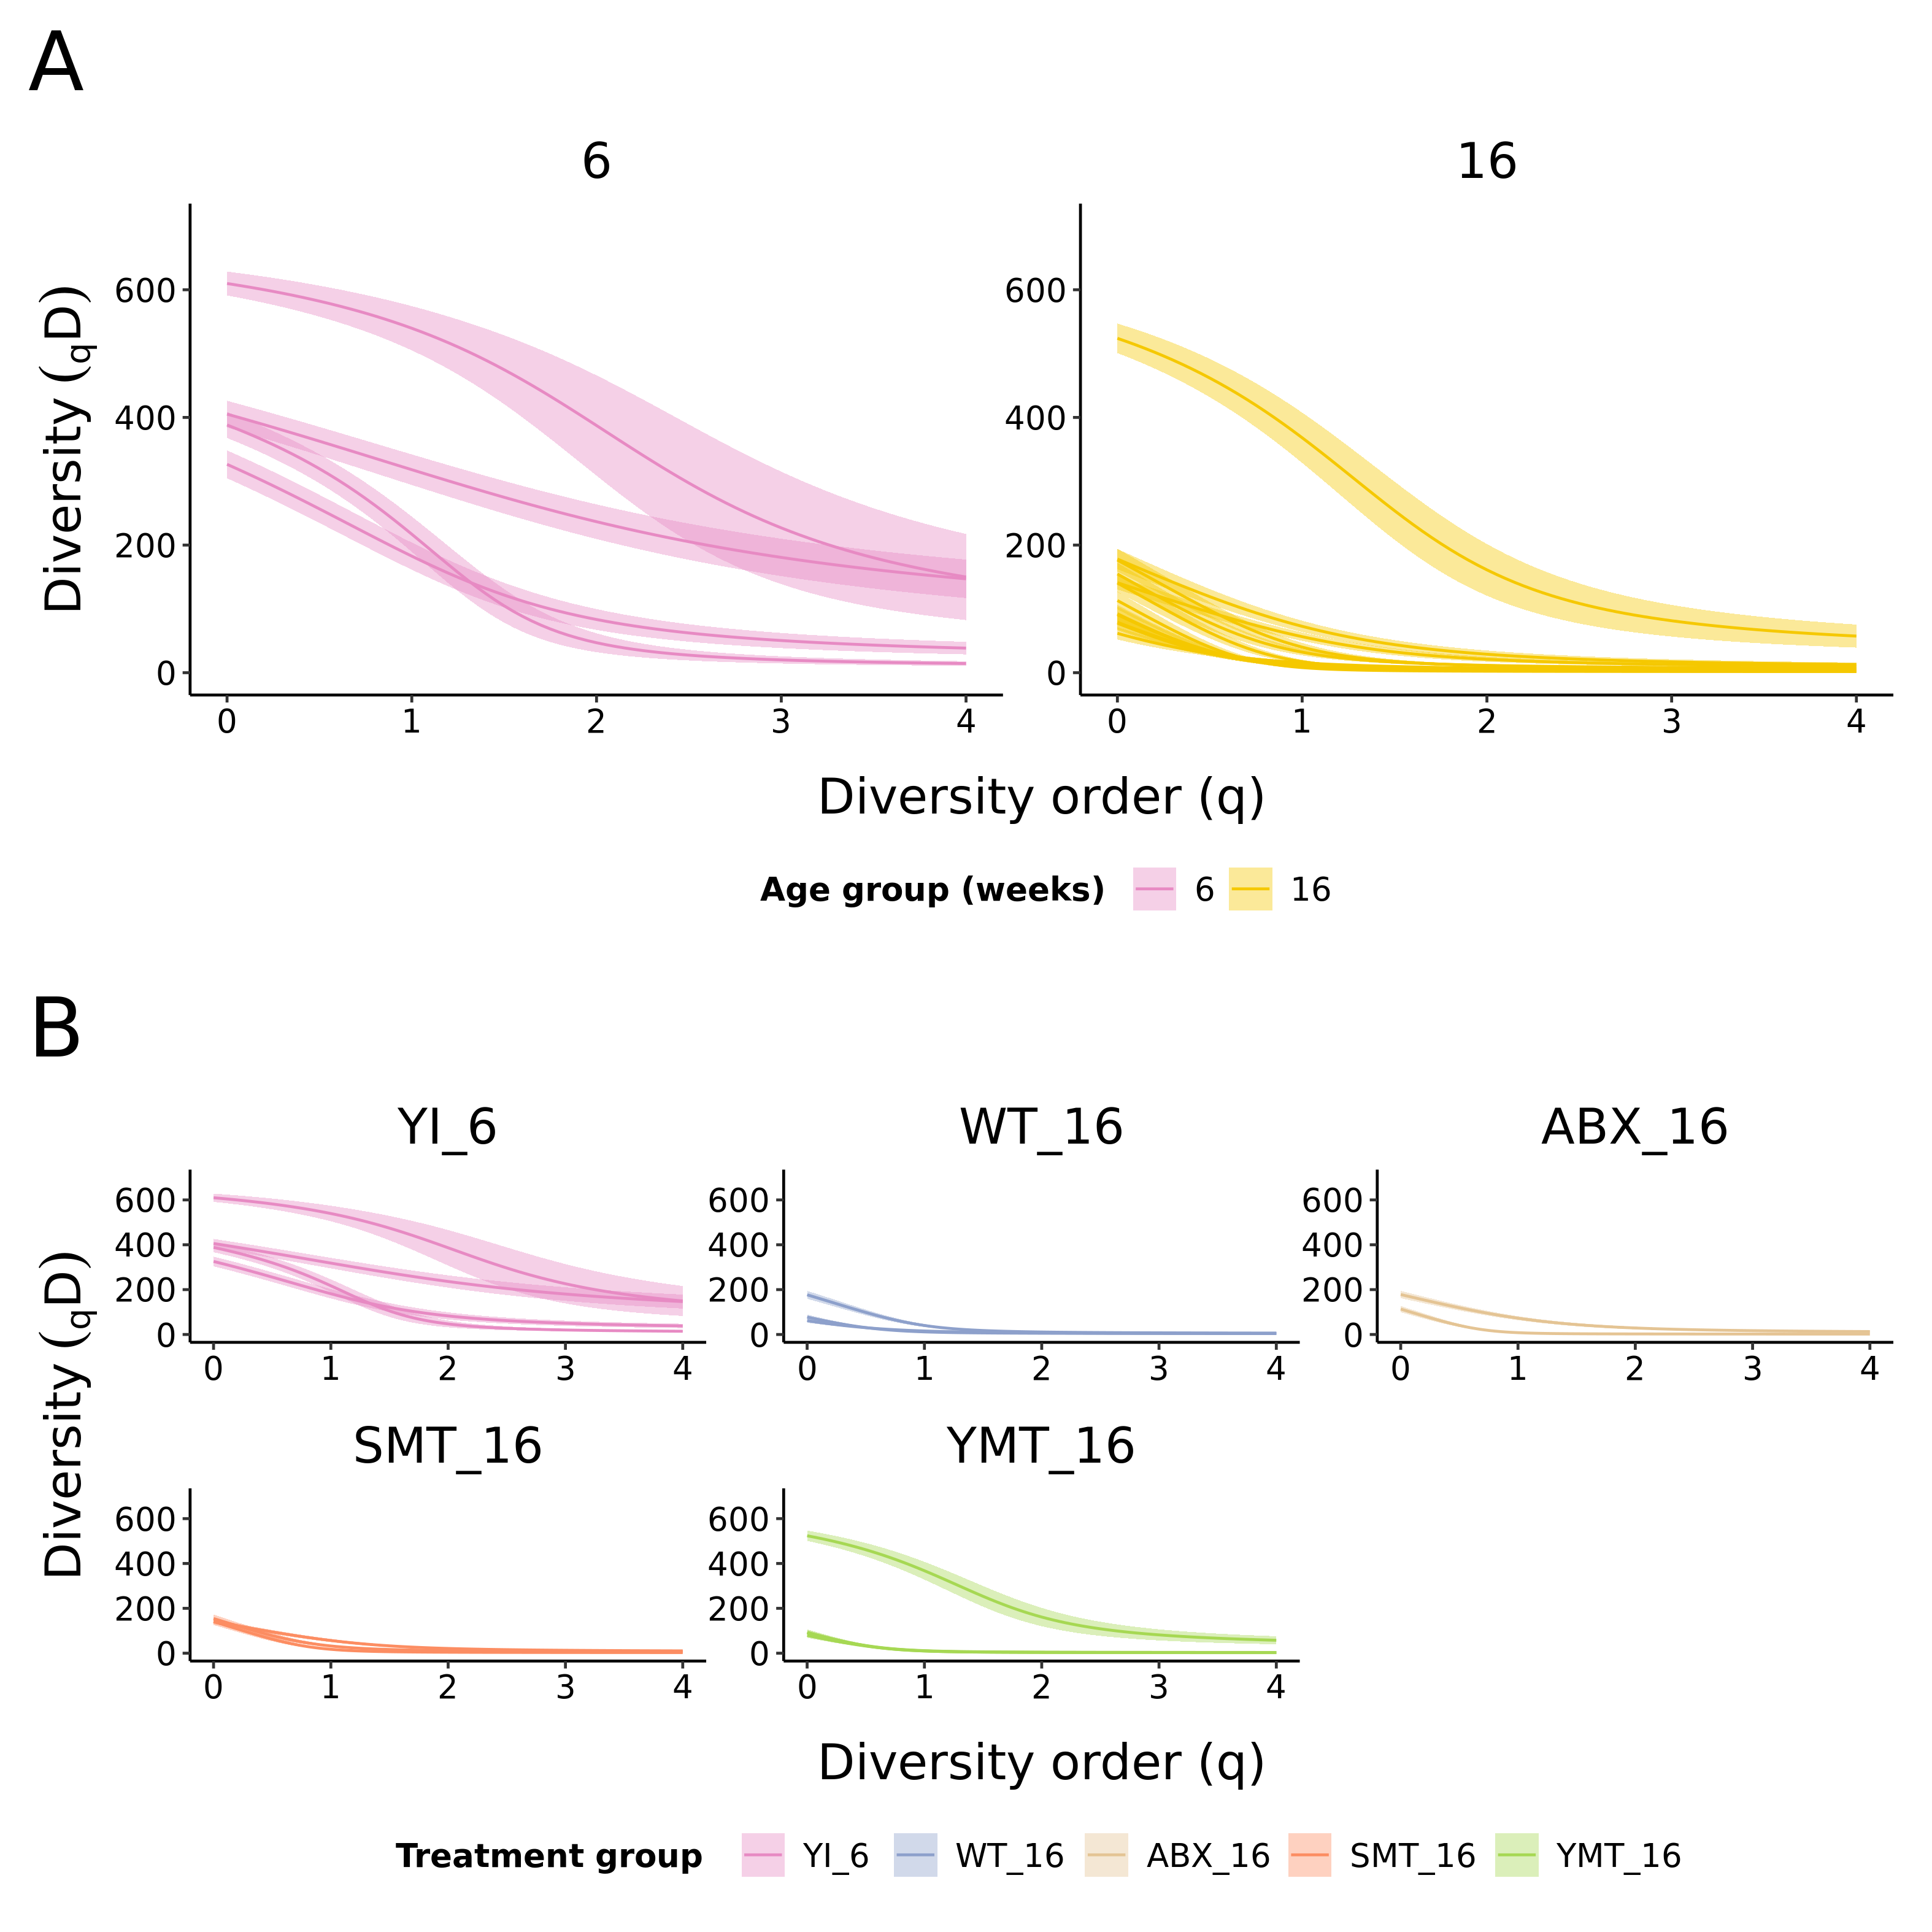
\includegraphics[width = 0.8\textwidth]{_Figures/png/igseq-gut-clone-diversity-solo-spectra}
\caption[Per-individual clonal diversity spectra for gut dataset]{\textbf{Per-individual gut diversity spectra for ageing dataset:} Hill diversity spectra of clone sizes (as measured by number of unique sequences per clone) for each individual in the \igseq gut dataset, grouped by (A) age at death and (B) treatment group.}
\label{fig:igseq-gut-clone-diversity-solo-spectra}
\end{figure}

\begin{figure}
\centering
\begin{subfigure}{0em}
\phantomsubcaption{}
\label{fig:igseq-gut-vj-diversity-solo-spectra-age}
\end{subfigure}
\begin{subfigure}{0em}
\phantomsubcaption{}
\label{fig:igseq-gut-vj-diversity-solo-spectra-groups}
\end{subfigure}
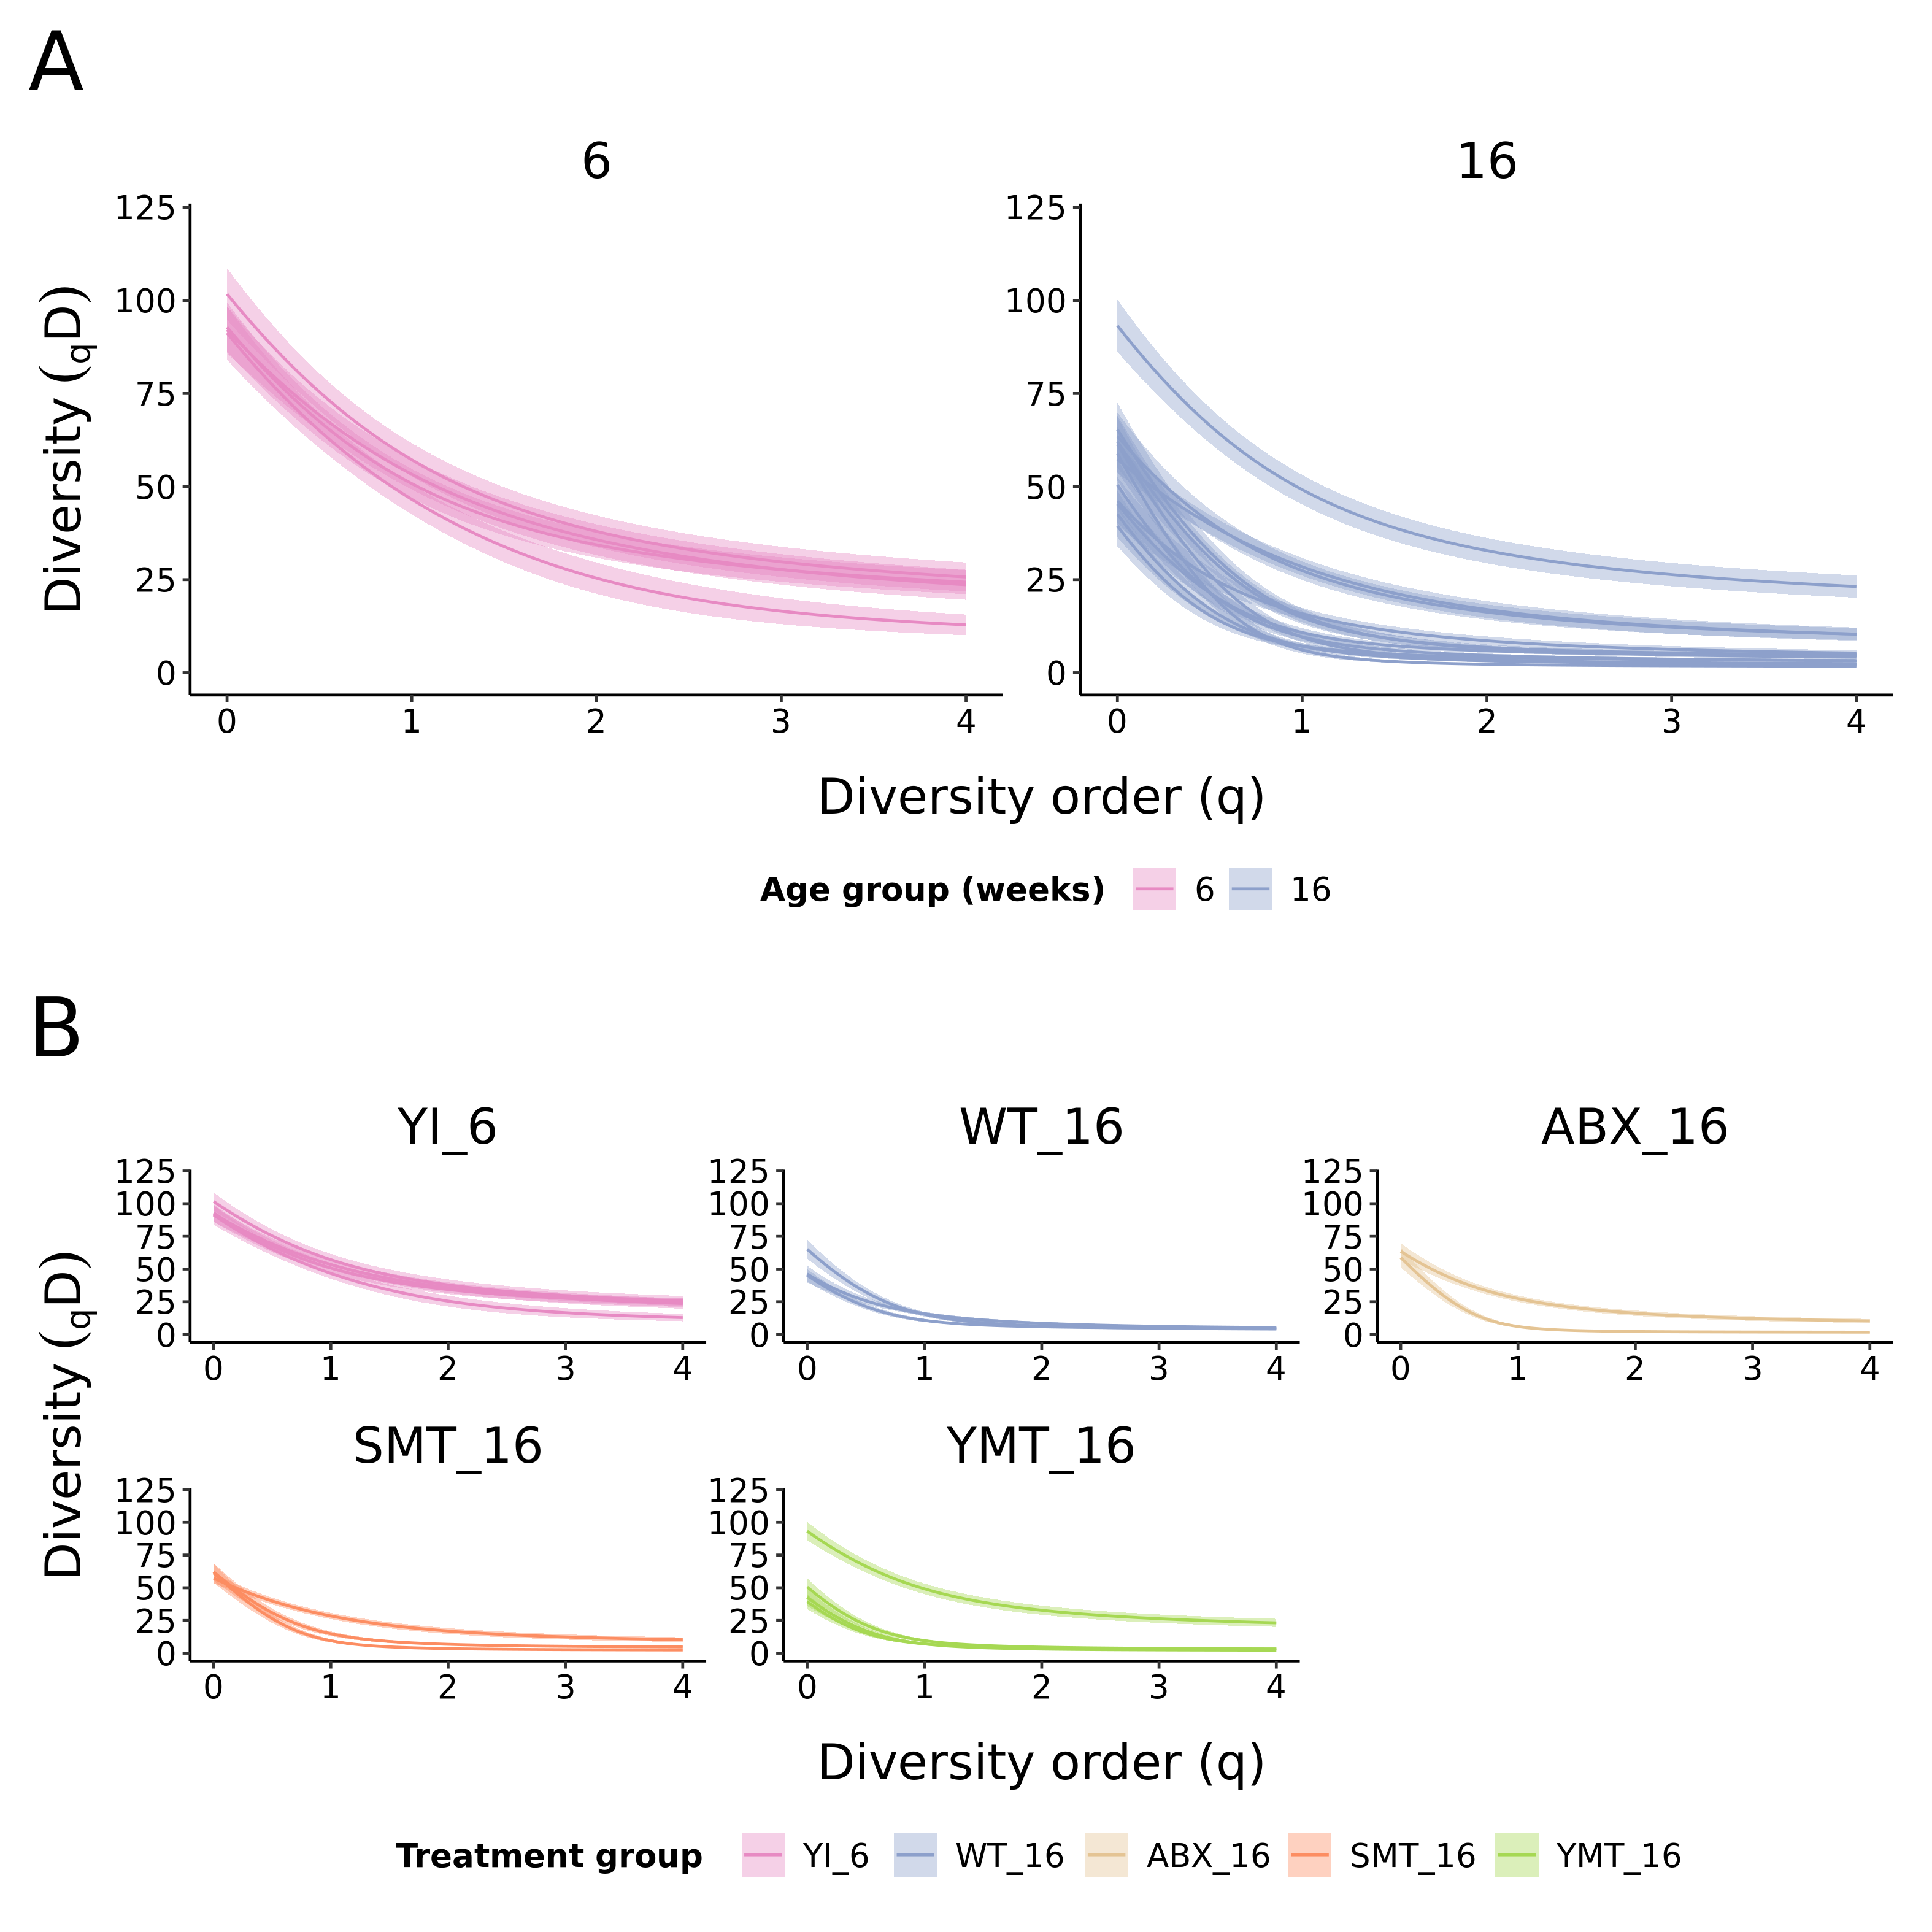
\includegraphics[width = 0.8\textwidth]{_Figures/png/igseq-gut-VJ-diversity-solo-spectra}
\caption[Per-individual VJ-diversity spectra for gut dataset]{\textbf{Per-individual VJ-diversity spectra for gut dataset:} Hill diversity spectra of VJ usage (as measured by number of unique sequences per V/J combination) for each individual in the \igseq gut dataset, grouped by (A) age at death and (B) treatment group.}
\label{fig:igseq-gut-vj-diversity-solo-spectra}
\end{figure}


\begin{figure}
\centering
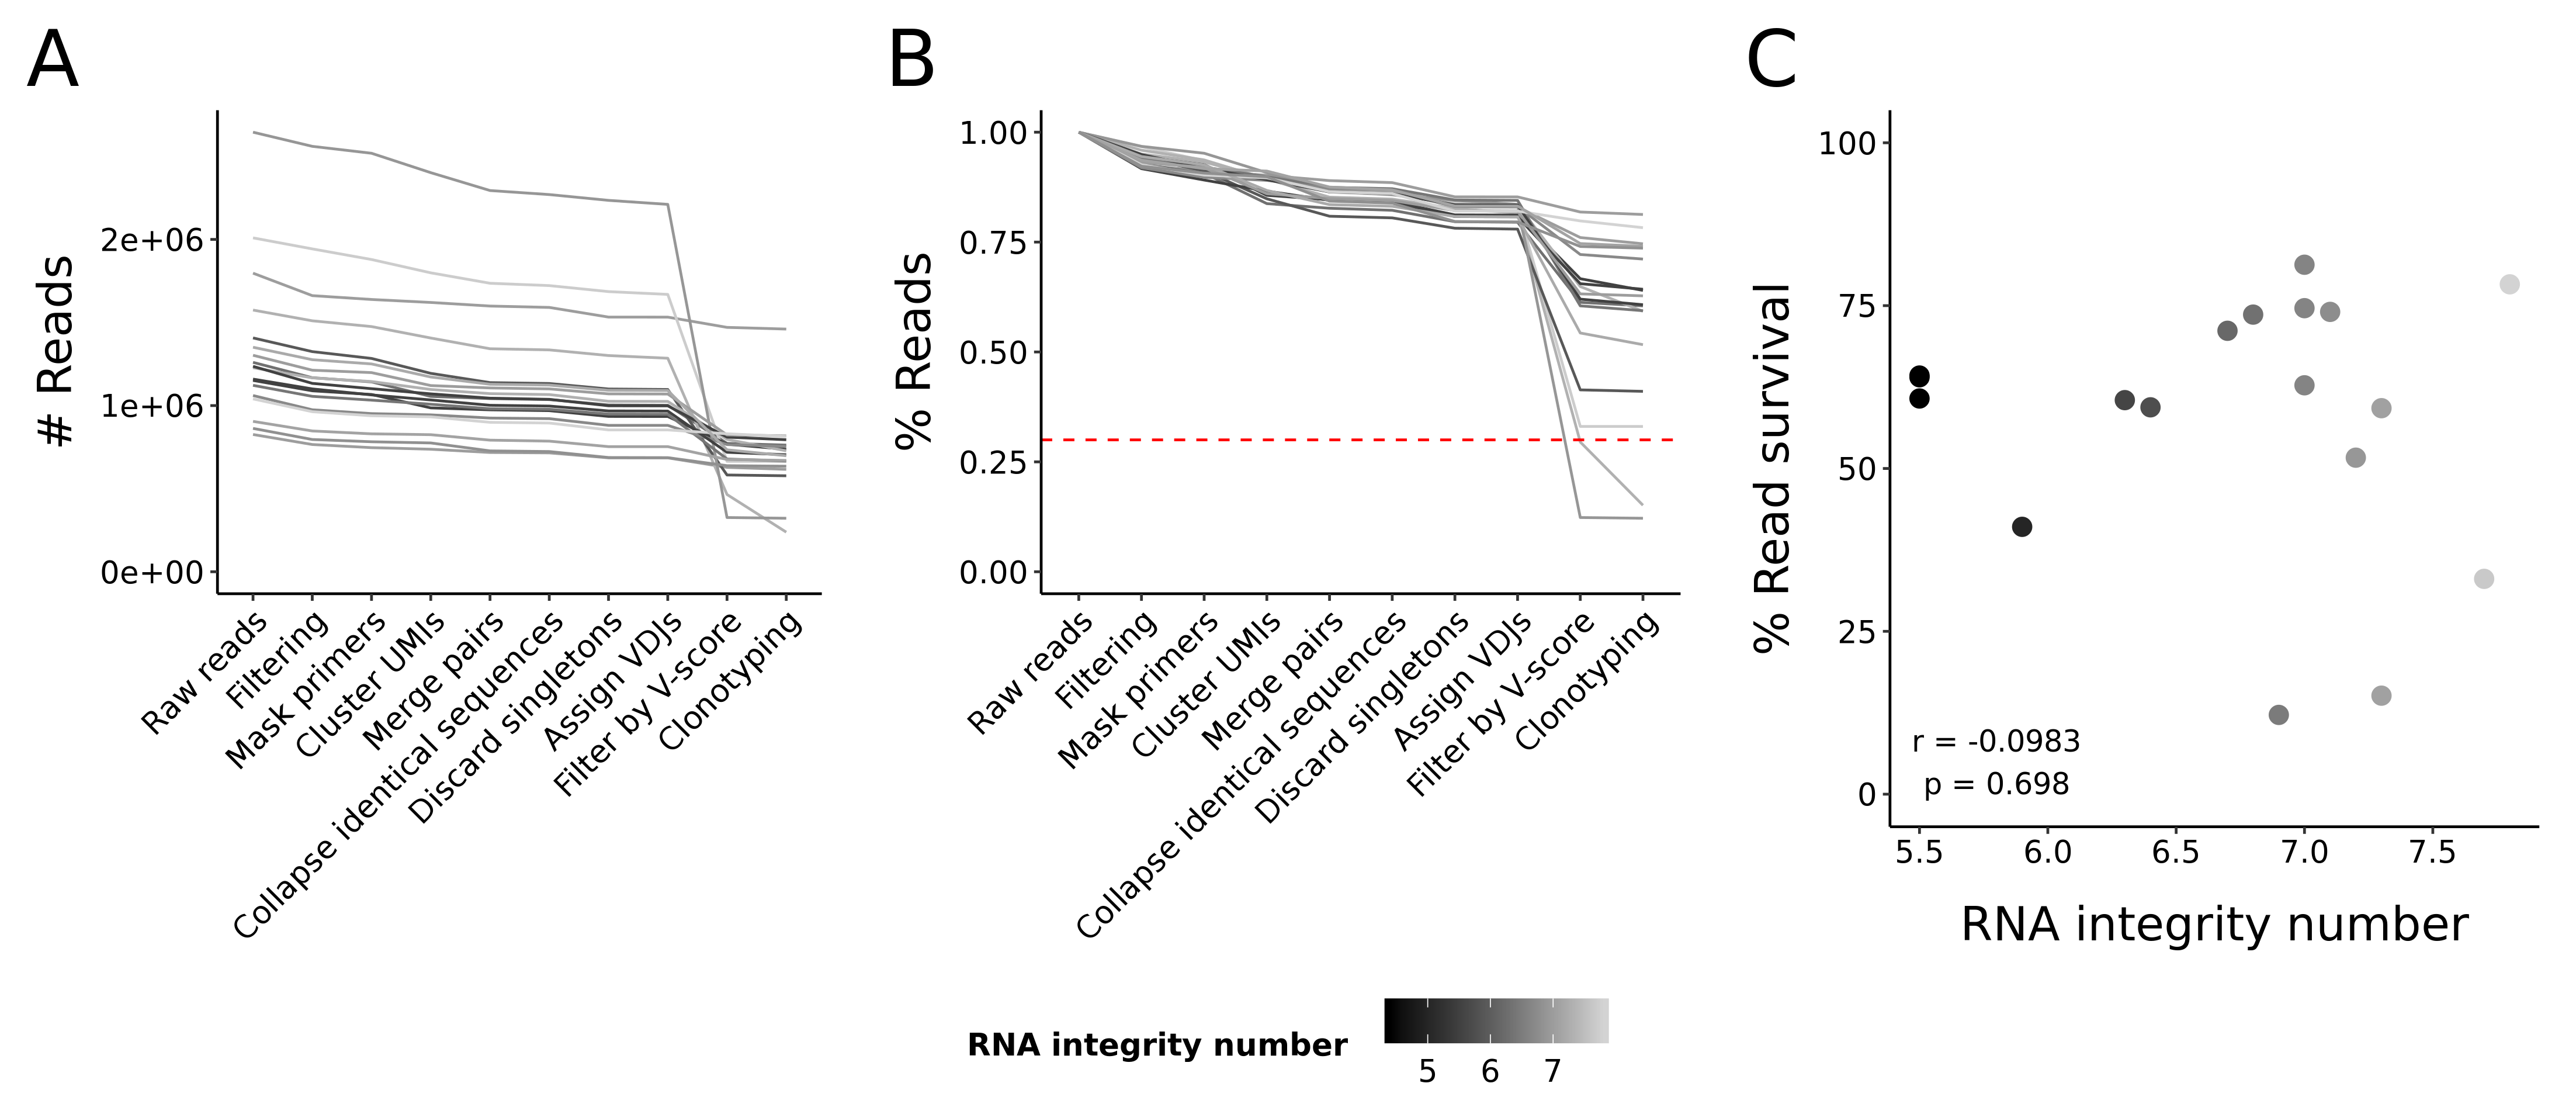
\includegraphics[width = \textwidth]{_Figures/png/gut-read-survival-all-rin.png}
\begin{subfigure}{0em}
\phantomsubcaption{}
\label{fig:igseq-gut-read-survival-all-rin-abs}
\end{subfigure}
\begin{subfigure}{0em}
\phantomsubcaption{}
\label{fig:igseq-gut-read-survival-all-rin-rel}
\end{subfigure}
\begin{subfigure}{0em}
\phantomsubcaption{}
\label{fig:igseq-gut-read-survival-all-rin-scatter}
\end{subfigure}
\caption[Relationship between RNA integrity and read survival in the gut \igseq dataset]{\textbf{Relationship between RNA integrity and read survival in the gut \igseq dataset:} (A-B) Absolute (A) and relative (B) read survival during pre-processing of the \igseq gut-microbiota-transfer dataset, up to and including clonotyping, coloured by the RNA integrity number of each input sample. The dotted red line in (B) indicates the 30\% read-survival cutoff, below which samples are discarded prior to downstream analysis. (C) Scatterplot of RNA integrity number \textit{versus} percentage read survival, up to and including clonotyping.}
\label{fig:igseq-gut-read-survival-all-rin}
\end{figure}